\documentclass[10pt, letterpaper]{article}
\usepackage[utf8]{inputenc}
\usepackage[left=1.5in,right=1in,top=1in,bottom=1in]{geometry}
\usepackage{pdfpages}
\usepackage{float}
\usepackage[backend=bibtex,citestyle=numeric-comp]{biblatex}

\usepackage{lipsum}
\usepackage{etoolbox}
\usepackage{subfig}

\usepackage[autostyle]{csquotes}
\addbibresource{references.bib}
\usepackage{lipsum}
\usepackage[doublespacing]{setspace}
\usepackage{indentfirst}
\usepackage{fancyhdr}
\usepackage{siunitx}
\usepackage{hyperref}

\usepackage{soul}
\usepackage[dvipsnames]{xcolor}
\DeclareRobustCommand{\Sid}[1]{{\begingroup\sethlcolor{green}\hl{(Sid:) #1}\endgroup}}

\linespread{2}
\begin{document}
\renewcommand{\thepage}{\roman{page}}
\begin{titlepage}
	\centering
	{\scshape\large Using molecular dynamics simulations to elucidate a role for bacterial ceramide \par}
	 By \par
	{\scshape\large Anushriya Subedy \par}
	 A thesis submitted to the \par
	 Graduate School-Camden \par
	 Rutgers, State University of New Jersey \par

	 In partial fulfillment of the requirements\par

	 For the degree of Masters of Science\par

	 Graduate Program in Computational \& Integrative Biology\par

	 Written under the directions of\par

	 Dr. Eric Klein and Dr. Grace Brannigan \par

	 And approved by\par
	
	\noindent\rule{8cm}{0.4pt}\par
	Dr. Eric Klein\par
	
	\noindent\rule{8cm}{0.4pt}\par
	Dr. Grace Brannigan \par
	
	\noindent\rule{8cm}{0.4pt}\par
	Dr. Guillaume Lamoureux \par
	
	

	\vfill
	Camden, New Jersey\par
	October 2021\par
% Bottom of the page	
\end{titlepage}

\newpage

\begin{abstract}
\setcounter{page}{2}
\phantomsection\addcontentsline{toc}{section}{Abstract}

% \center THESIS ABSTRACT\par
\center Using molecular dynamics simulations to elucidate a role for bacterial ceramide\par
\center by Anushriya Subedy\par
\center Dissertation Directors:\par
\center Dr. Eric Klein and Dr. Grace Brannigan\par 
\bigbreak

\bigbreak

\bigbreak

\begin{flushleft}Sphingolipid synthesis was thought to be rare in Gram-negative bacteria, previously only found in a handful of taxa. We recently discovered
ceramides in \textit{Caulobacter crescentus} and demonstrated that these lipids play an important role in antibiotic and phage sensitivity. However, the mechanism by which ceramides affect resistance to antimicrobials, as well as their effects on the integrity of the cell membrane is not yet clear. In this study, a coarse-grained molecular dynamics simulation of a prototypical bacterial outer membrane is used to observe changes in the structure of the outer membrane lipids in the presence of ceramides. The outer membrane of a Gram-negative bacteria is asymmetric with an outer leaflet dominated by lipopolysaccharide (LPS). LPS is composed of three domains that extend from the outer membrane: (1)~a membrane-embedded lipid A, (2)~the attached core polysaccharide chain, and (3)~the O-antigen polysaccharide chain. There are two variants of LPS, rough LPS (RLPS) consists of lipid A and the core sugars only, while smooth LPS (SLPS) has additional O-antigen chains. To understand the role of ceramides in outer membrane structure and function, this study considers the ceramide-mediated effects on the clustering and packing of LPS and membrane lipids. Our findings suggest a ceramide concentration mediated effect on LPS packing. The area per lipid increases with increasing ceramide concentration. Additionally, ceramide preferentially interacts with the more disordered domain. Ceramide disrupts the ordered domain while ordering the disordered domains.  

\end{flushleft}. 

\end{abstract}
\newpage


\newpage
\tableofcontents
\newpage

\cleardoublepage
\phantomsection\addcontentsline{toc}{section}{\listfigurename}
\listoffigures

\clearpage
\pagenumbering{arabic}
\pagestyle{myheadings}

\section{Introduction}

\fancyhf{}
\fancyhead[R]{\thepage}

Cell membranes form a semi-permeable biological barrier in living systems to separate the chemical reactions needed for life from the surrounding environment. Biological membranes are composed of mixtures of lipids and associating proteins. Lipids are amphiphilic, meaning they contain a hydrophilic headgroup and one or more hydrophobic fatty acid acyl chains. Lipids are organized with the non-polar fatty acid tails tucked inside a protective hydrophobic region while the polar headgroups contact the cytoplasm and the extracellular environment, creating a bilayer membrane.
The most commonly found lipids in membranes include glycerophospholipids with glycerol backbone that  connect the headgroup, with varying size and charge, with the tail(s) \cite{botan2015toward}. The hydrocarbon tails can also vary by the number of carbons and the number of tails, ranging from two to eight, across the eukaryotic and prokaryotic domains \cite{kim2016bilayer}. A typical characteristic of eukaryotic lipids is having two acyl chains each with an even number of carbon atoms (Figure \ref{fig:structure}). However, bacterial lipids may contain more than two fatty acid chains and typically have an odd number of carbon atoms in the hydrocarbon  chains \cite{kim2016bilayer}. The acyl chains can be unsaturated or saturated, which is indicated by the presence or absence of double bonds, respectively.
The double bonds cause \enquote{kinks} in the acyl chains which can further impact the packing of lipids in the membrane. 

\par The typical landscape of a eukaryotic membrane consists of a single bilayer composed of phospholipids. Meanwhile, bacteria are classified into two groups, Gram-positive and Gram-negative, based on the structure of their cell envelope. Gram-positive bacteria have a single phospholipid bilayer surrounded by a thick peptidoglycan layer. The cell envelope of Gram-negative bacteria is composed of an inner and an outer membrane, that are separated by a thin peptidoglycan layer. The asymmetric outer membrane is composed primarily of a complex lipid, lipopolysaccharide (LPS), which is made up of three domains: (1)~lipid A, (2)~core oligosaccharide, and (3)~O-antigen chain \cite{rittig2003smooth}. The hydrophobic lipid A containing phosphate groups, hexosamines, and fatty acid chains, anchors to the outer leaflet of the outer membrane. The core oligosaccharide chain attaches to the lipid A and consists of repeating units of sugars such as keto-deoxyoctulosonate (KDO) and hexoses such as glucose and mannose. Attached to the core, via ligation to hexose sugar units, is the O-antigen, which is made up of several repeating sugar subunits.  
Among LPS containing Gram-negative bacteria, there is great diversity in the makeup of the LPS components. Lipid A is a conserved moiety, however, the number of acyl chain vary among species. For instance, the lipid A of \textit{Escherichia coli} is hexa-acylated, while \textit{Serovar typhimurium} lipid A is hepta-acylated \cite{scott2017lipid, kong2012phosphate}.
The O-antigen composition and length vary greatly between species. 
The variability in the composition of LPS further increases the complexity of the outer membrane structure. Furthermore, the LPS is separated into two types, smooth LPS (SLPS) and rough LPS (RLPS) based on the presence of the third domain, the O-antigen chain. SLPS contains all three domains, while RLPS lacks the O-antigen chain. In addition to the LPS, the outer membrane also includes phospholipids, such as phosphatidylglycerol (POPG). In contrast to the complex outer membrane, the symmetric inner membrane is composed primarily of phospholipids, similar to a eukaryotic membrane.

\begin{figure}[H]
  \centerline{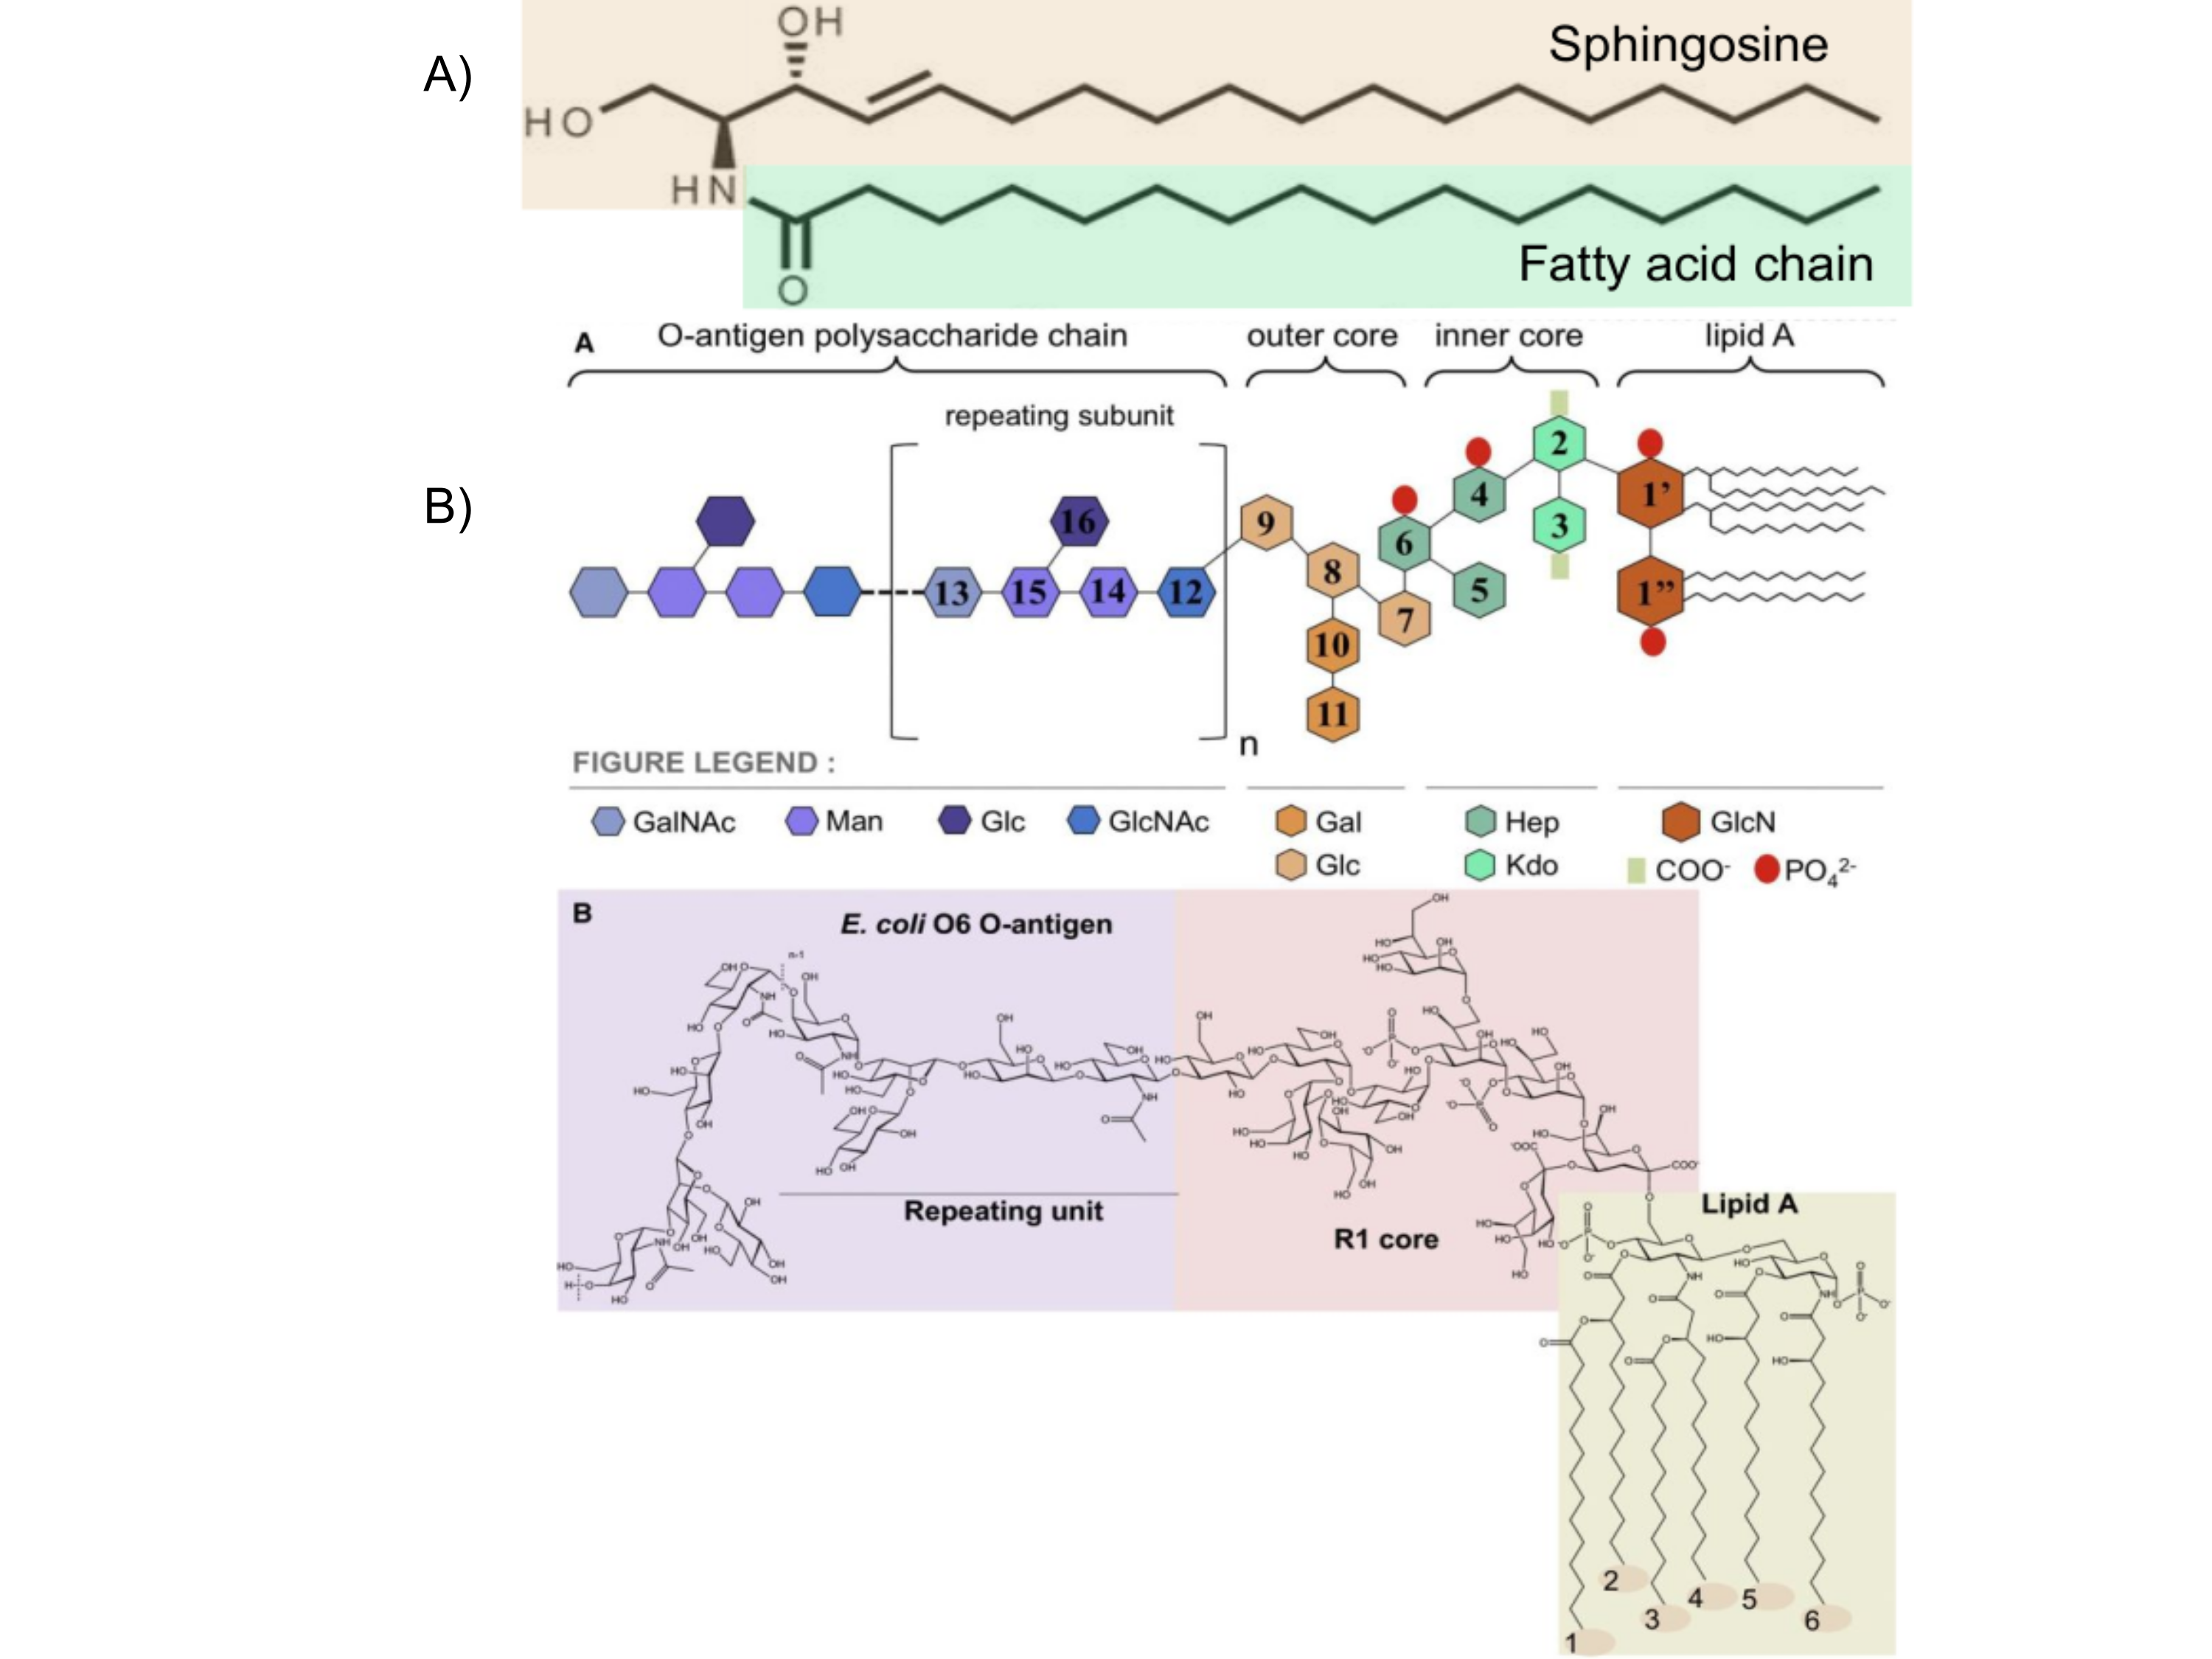
\includegraphics[width=\textwidth, scale=0.85]{MS thesis/figures/intro_structure.png}}
  \caption[Structure of Lipids]{Chemical structure of ceramide and \textit{E. coli} LPS: (A) ceramide (d18:1/16:0). Sphingosine backbone is highlighted in orange and the fatty acid chain is highlighted in green. (B) \textit{E. coli} LPS, showing the three domains, lipid A, R1 core and O-antigen chain, image taken from Wu et al.\cite{wu2013molecular}. Lipid A acyl chains are numbered, 1-6 from left to right \cite{becam2017antibacterial, wu2013molecular}.}
  \label{fig:structure}
\end{figure}

\par Besides the commonly found phospholipids, certain Gram-negative bacteria such as \textit{Sphinogmonas}, can synthesize sphingolipids. Although sphingolipids are rare in  Gram-negative bacteria, they are commonly found in eukaryotic membranes, where sphingolipids play an important role in signaling and cell recognition \cite{alonso2018physical, veiga1999ceramides,zhang2009ceramide}. Sphingolipids differ from phospholipids as they contain an amino alcohol backbone, the sphingoid base, instead of a glycerol backbone. There are many derivatives of sphingolipids, such as ceramide, which only contain a fatty acid chain connected to a sphingosine backbone, (Figure \ref{fig:structure}) \cite{alonso2018physical, zhang2009ceramide}. Ceramides in eukaryotic membranes exhibit certain unique properties such as increasing the order of the membrane and inducing domain formation \cite{alonso2018physical, veiga1999ceramides}. 
\par Lipids can separate into two phases, liquid ordered ($\rm L_o$) and liquid disordered ($\rm L_d$). Liquids in each domain have specific defining characteristics. The liquid ordered phase is typically enriched in saturated and tightly packed lipids with a large order parameter. In eukaryotic membranes, $\rm L_o$ domains are enriched in cholesterol or glycosphingolipids. The concentration of cholesterol affects membrane phase transitions and domain formation. For instance, the order of the membrane increases with increasing cholesterol concentration, and the area per saturated lipid decreases, typically with change in phase occurring at about 15\% cholesterol. \cite{wang2016dppc}. The liquid disordered phase contains unsaturated lipids that are loosely packed. The area per lipid within the $\rm L_d$ phase is larger in contrast to the small area per lipid found in the $\rm L_o$ phase \cite{van2008membrane}. Interactions of lipids influence the membrane by inducing phase separation of lipids, creating microdomains within the membrane.


\par The role of sphingolipids in bacterial membranes is not yet clear. In some Gram-negative species, such as in \textit{Sphingomonas}, sphingolipids take the place of LPS in the outer membrane \cite{kawasaki1994cell}. In \textit{Porphyromonas gingivalis} sphingolipids play a role in pathogenesis, specifically in manipulating host immune response \cite{rocha2020porphyromonas}. Additionally, a recent study by Stankeviciute et al., \cite{stankeviciute2019caulobacter}, has shown that \textit{Caulobacter crescentus}  produces a novel glycosphingolipid under phosphate starvation. Interestingly, \textit{C. crescentus} can synthesize neutral ceramide under a range of phosphate conditions \cite{stankeviciute2019caulobacter}. Furthermore,  \textit{C. crescentus} deficient in ceramide are resistant to polymyxin B, a commonly used antibiotic against Gram-negative bacteria, and the cells became more susceptible to bacteriophage infection. The mechanisms by which ceramide influences antibiotic and phage sensitivity are not yet known. These observations have motivated us to study the role of ceramide in bacterial membranes. 


\par It is a challenging task to study bacterial membranes experimentally due to the lack of experimental techniques needed to stain or extract LPS with unknown O-antigen moieties, such is the case of \textit{C. crescentus}. Furthermore, the \textit{C. crescentus} cell envelope includes a multiplex surface protein layer,(S-layer) that is attached to the LPS. The S-layer introduces additional layer of complexity in understanding the interactions of lipids within the membrane, experimentally. Instead, \textit{in silico} methods such as  Molecular Dynamics (MD) simulations, both all-atom and coarse-grained, have been used to study outer membrane lipids. All-atom MD simulations allow for finer resolution study of the system, albeit at a short nanosecond time scale. Although coarse-grained simulations have reduced resolution, they can be run at a longer, microsecond time scale allowing us to study the structural changes occurring within the membrane.

\par Considerable progress has been made in studying the properties of gram-negative bacterial outer membranes using MD over the last decade. All-atom simulations of \textit{E. coli} outer membrane involving various lengths of SLPS ranging from zero to ten sugar residues in a mixed system with RLPS shows that the longer the length of O-antigen, the less it was extended. This suggests that the terminal residues are more dynamic in contrast to the internal residues due to the difference in packing \cite{wu2013molecular}. The area per lipid increases as the core sugars and the O-antigen domains are added. This is due to the steric hindrance caused by the bulky sugar subunits of the O-antigens which \enquote{push} individual LPS molecules further apart \cite{wu2013molecular}. The area per lipid of LPS is further influenced by the number of acyl chains in lipid A; such that the area increases as the number of the chain increases \cite{kim2016bilayer}. In addition to packing, the dynamics of LPS suggest that the LPS is largely immobile and has a slow diffusion rate, as compared to other phospholipids \cite{patel2016dynamics, lopez2020molecular}. 
One method of studying the fluidity of a membrane is by conducting an order parameter calculation. The addition of core sugars and the length of O-antigen affect the order of the LPS molecule. LPS containing lipid A alone shows the highest order and smallest area per lipid.  While the addition of core sugars and O-antigen decreases order and subsequently increases the area per lipid, which further suggests a fluid behavior of the LPS \cite{wu2013molecular}. 
\newpage
\par A recent coarse-grained MD study by  Jefferies et al reports several novel observations of the LPS structure and dynamics \cite{jefferies2019role}. From simulations containing SLPS alone and SLPS in mixed membrane with RLPS and other phospholipids, the authors find that the orientation and packing of LPS depend on its environment. In simulations with SLPS alone, the O-antigens conform to a lamellar packing. In a mixed environment, the O-antigen chains become more disordered. Additionally, the O-antigen tilts significantly in a mixed environment as compared to when SLPS is alone in the system. This suggests LPS, particularly the O-antigen clustering is a favorable process within mixed systems. Furthermore, the SLPS mobility is increased when RLPS or phospholipids are in proximity. 

\par Although properties of a bacterial outer membrane have been studied, it is not yet clear how the addition of unique bacterial lipids such as ceramide affects the overall lipid interactions and membrane structure. This present study uses coarse-grained MD using a prototypical LPS from \textit{E. coli} to better understand how the membrane properties are affected by incorporating a range of ceramide concentrations from 0-25\%. We hypothesize that the presence of ceramide induces domain formation further affecting the structure of the outer membrane.


\newpage
\section{Methods}

\subsection{Membrane setup}
Randomized membranes were built using CHARMM-GUI  Martini Maker \cite{hsu2016molecular, shearer2019outer}. For each membrane, the outer leaflet contained 1:1:0.5:X of SLPS (OANT), RLPS (RAMP), POPG, DPCE respectively. The X indicates the concentrations of ceramide, (DPCE C(d18:1/18:0)), of 0\%, 5\%, 10\% and 20\%.  The inner leaflet contained a 95:5 ratio of POPG (C16:0/18:1 1-palmitoyl-2-oleoyl) and diacylglycerol (PODG) (Figure \ref{fig:intro}A, B). \textit{E. coli} LPS was used as a representative of a prototypical LPS given its availability for coarse-grained simulations. Three independent initial inputs were generated from CHARMM-GUI for each of the four ceramide concentration systems. 

\par The artificial membrane was created by combining two separate bilayers generated using  CHARMM-GUI Martini Maker: 1)~a large 20x20 $\rm nm$ bilayer where the outer leaflet consisted of only  RLPS was generated and 2)~a smaller 10x10 $\rm nm$ membrane containing only SLPS in the outer leaflet. The SLPS membrane was then inserted into the larger RLPS membrane using VMD (Figure \ref{fig:intro}C, D). First, the two systems were centered and overlapped using qwrap \cite{jerome_henin_2020_3877030}. In the outer membrane, a hole was cut out based on the maximum and minimum X, Y dimension of the smaller membrane. Each membrane was saved independently then merged, where any overlapping and incomplete lipids were removed to produce the final membrane.
A new topology file was generated for the membrane by selecting the names of the lipid in the order as it appears in the final merged pdb file using a bash script. Appropriate topology headers were added. After the minimization step, the charge of the system was examined. If the system contained a non-zero charge, neutralizing ions were removed from the pdb file as needed. Four simulations with the following concentration of ceramide were built; 0\%, 10\%, 15\%, and 20\% 25\%. Three replicate simulations were run for each of the five simulations.


\begin{figure}[H]
  \centerline{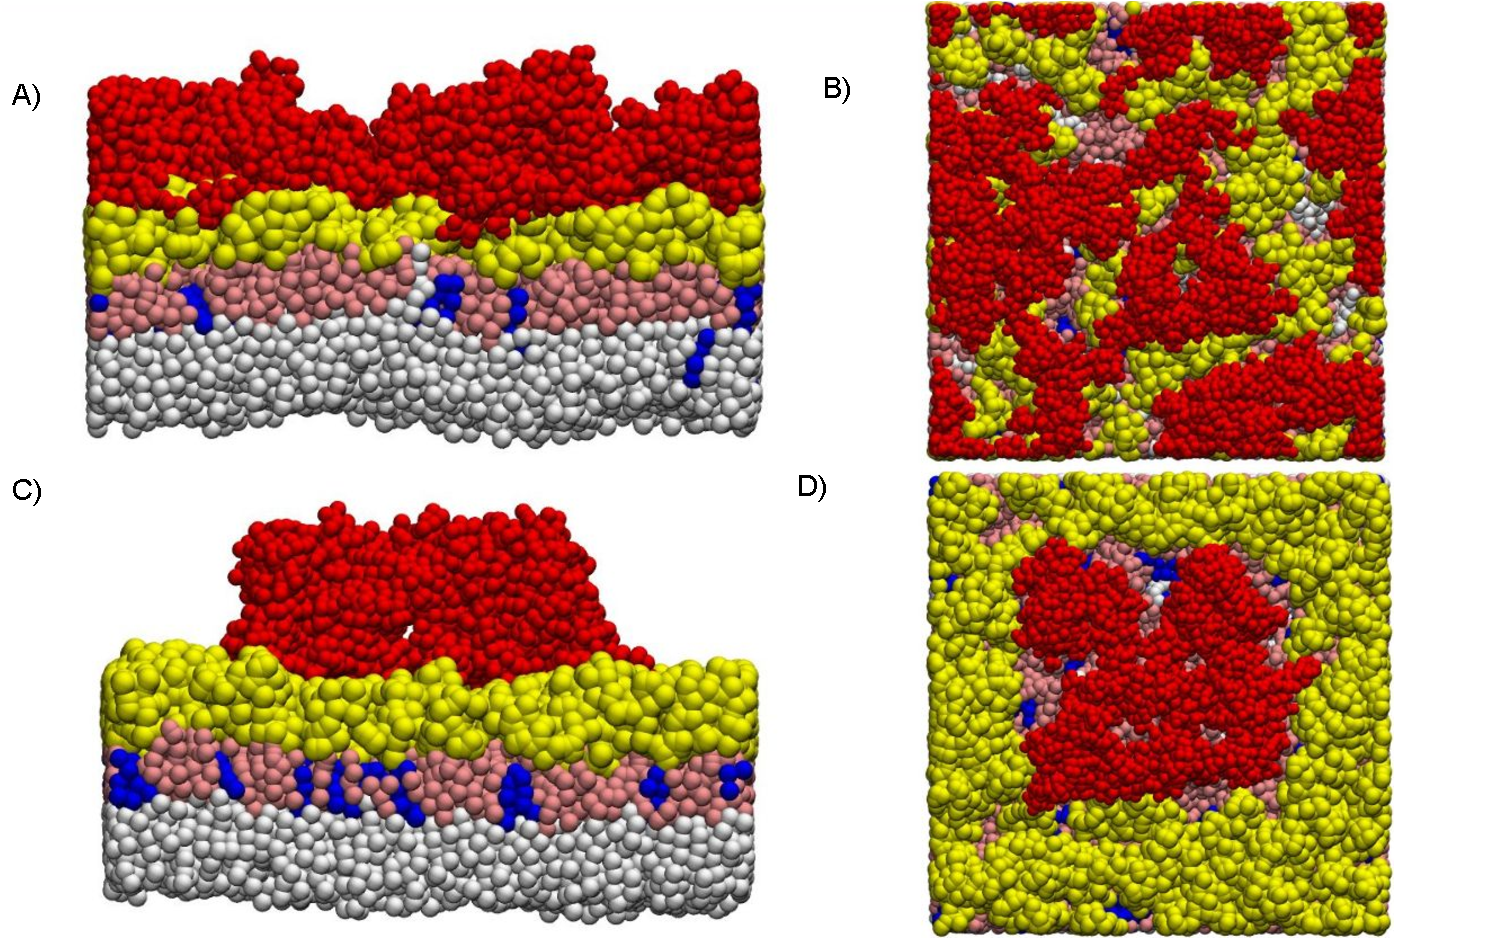
\includegraphics[width=11cm, scale=0.75]{MS thesis/figures/intro_combined2.pdf}}
  \caption[Random and Artificial outer membrane System set up]{Outer membrane simulation set up. A randomized membrane and an artificial membrane set up are depicted on top (A, B) and bottom (C, D) panels, respectively. Side profiles of the membranes are on the left and extracellular views are on right. Ceramide is only present in the outer leaflet of the outer membrane.
  The color scheme for the lipids is the following: white represents POPG in the inner leaflet. In the outer leaflet, ceramide is colored in blue, LPS is split up into three domains with lipid A in pink, core sugars in yellow, and the O-antigen chain in red.}\label{fig:intro}
\end{figure}

\subsection{Simulation setup}
The randomized and the artificial membranes were run using Gromacs 2016 and 2019 respectively \cite{abraham2015gromacs}. Both systems were run with Martini 2.2 Force Field  \cite{marrink2007martini}. Both systems were minimized using the steepest descent gradient. Following minimization, the randomized system and the artificial systems were equilibrated for 100$\rm ns$ and 200$\rm ns$ respectively. The production steps were run for 40 and \SI{20}{\micro\second} at 0.020$\rm ps$ time-step for randomized and artificial systems, respectively. Simulations were run using an isothermal-isobaric (NPT) ensemble. Pressure and temperature were kept constant for all simulations. For both systems, the temperature was set to 323K with velocity rescaling. Parrinello-Rahman, semi-isotropic pressure coupling with reference pressure set to 1.0 bar.

\subsection{Analysis}
Simulations were visualized and imaged using Visual Molecular Dynamics (VMD)\cite{humphrey1996vmd}. Radial distributions were calculated using Gromacs radial distribution (rdf) tools \cite{abraham2015gromacs}. Radial distribution was calculated for 2D (X and Y) dimensions, by selecting only a central bead (GM2) within lipid A backbone. Order parameter was calculated using equation \ref{Eq:order}. $\theta$ represents the angle between each of the acyl chain vector and bilayer normal, (Z-axis), averaged over time and all the reference lipids. \cite{piggot2017calculation}. Gromacs built-in Order parameter tool was used to calculate LPS order for each of the six acyl chains independently.


\begin{equation}
\label{Eq:order}
\mathrm{S} = \langle 3(cos\theta)^2 -1 \rangle /2
\end{equation}

The radius of gyration was calculated for LPS lipid A using equation
\ref{Eq:rgyr}, by taking the sum over all the position (i) of lipid A subtracted from the center of mass ($\rm x_0$, $\rm y_0)$, of each lipid A at each time point. Then, divided by the total number of beads in lipid A (N), and averaged over all lipids and over the last \SI{20}{\micro\second} of simulation time.
\begin{equation}
\label{Eq:rgyr} %$a_{bc}$
\sum[(x_{ij}-x_{0j})^2+(y_{ij}-y_{0j})^2]/N
\end{equation}

Ceramide-lipid A interaction enrichment was calculated by first measuring the distance between each position along the acyl chains of ceramide and lipid A (see Figure \ref{fig:bond}), using VMD measure bond tool. Ceramide is able to flip to the lower leaflets, thus, in this analysis, only ceramide in the upper leaflets at given time point was considered. Ceramide and lipid A within 8\si{\angstrom} were considered. For each of these pairs, distance along each positions were calculated. Distances larger than 10\si{\angstrom} were removed. Enrichment was calculated by dividing the percentage for each interaction site by the null hypothesis value, which states the probability of all position pairs having equal interaction, without any selection. The null hypothesis was calculated by taking the total position of lipid A (32) and multiplying by the total position of ceramide (9) to get a value of 288 or 0.34 represented as a percent.
\begin{figure}[H]
  \centerline{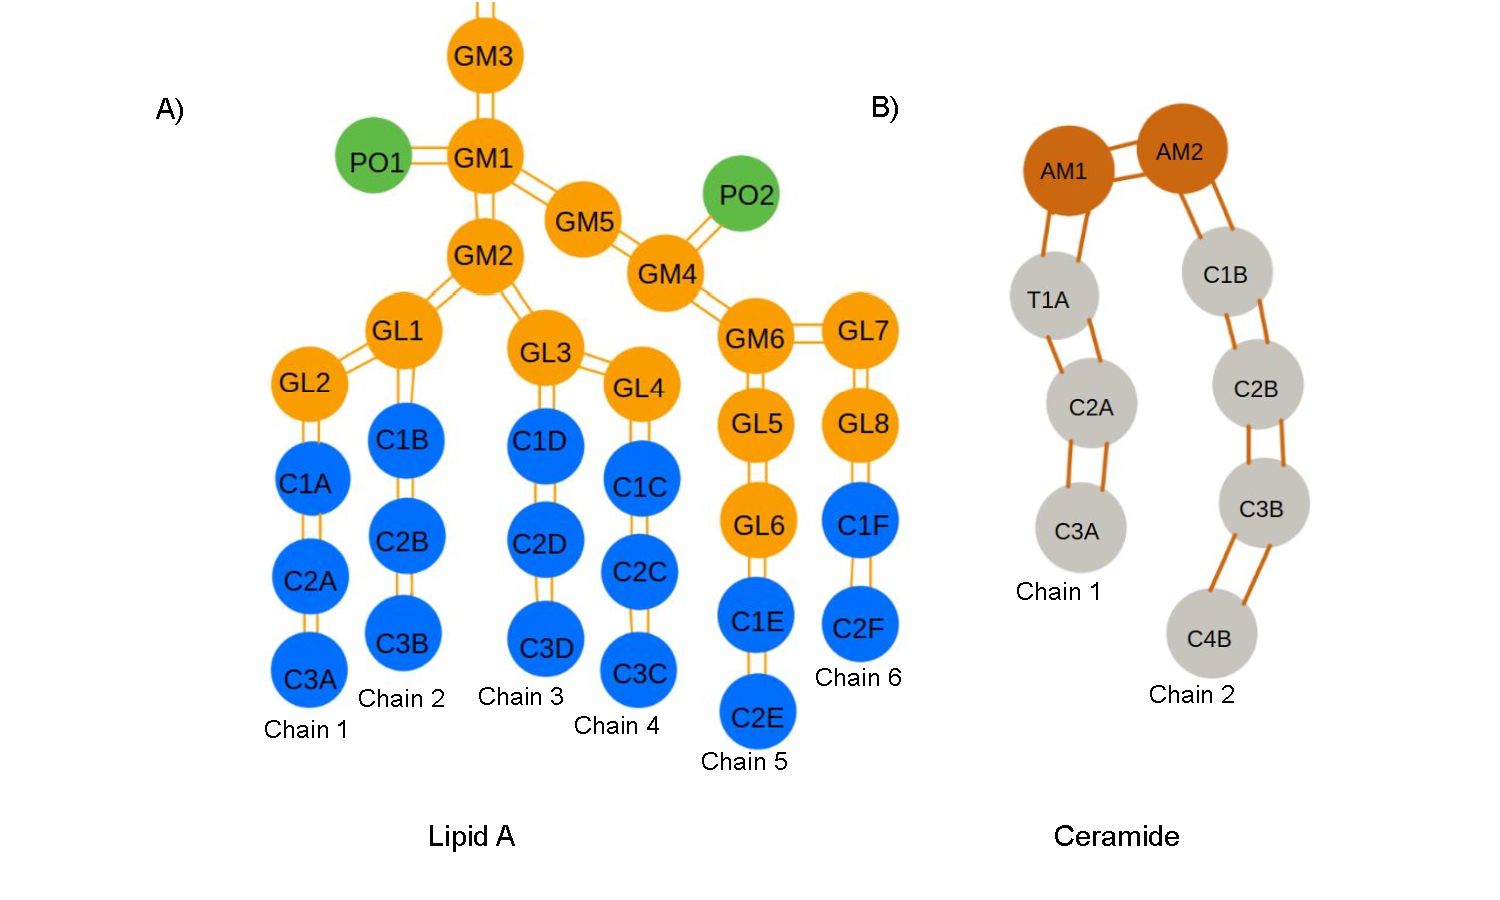
\includegraphics[width=11cm, scale=0.75]{MS thesis/figures/bond_measure_chain_label.pdf}}
  \caption[Coarse-grained ceramide and lipid A structure]{Coarse-grained structure of Lipid A and ceramide with positions labeled using martini bead nomenclature. Each sphere represents a single position along the chain. a) Lipid A: phosphate groups are colored green, sugar groups in the backbone are colored in orange, acyl chains are colored in blue. b) Ceramide (DPCE): Acyl chains are colored in gray. Chain 1 represents the unsaturated tail, chain 2 represents the fully saturated tail \cite{marrink2007martini, hsu2016molecular}. }
  \label{fig:bond}
\end{figure}

In the artificial membrane, ceramide occupancy was calculated in three regions, RLPS, SLPS, and the boundary region (Figure \ref{fig:number_cer}). The boundary region was measure by selecting SLPS within 4.7\AA~of RLPS, and RLPS within 4.7\AA~of SLPS. A cut-off distance of 4.7\AA~ was set between ceramide and given LPS. Selections were made such that ceramide is only counted once within a specified region. Percent ceramide occupancy was calculated over \SI{20}{\micro\second}. Enrichment was calculated by taking the percent of ceramide in each region and diving by the expected percent in each domain if ceramide was randomly distributed. For instance, the expected percent was calculated in the RLPS region by counting the number of RLPS in the region minus RLPS in boundary divided by the total number of LPS in the system. SLPS normalization was calculated similarly. For the boundary, only RLPS and SLPS within the given cut-off distance were selected, and divided by the total number of LPS.


\newpage
%% RESULT SECTION
\section{Results}
\subsection{Randomized Membrane}
\par The randomized membrane represents a native bacterial membrane topology, where lipids are not initialed at specific positions (Figure {\ref{fig:intro}}). Four simulations were performed with the following compositions: 1:1:0.5 ratio of SLPS, RLPS, POPG respectively, with ceramide concentrations of 0\%, 5\%, 10\%, and 20\%. A wide range of concentrations was incorporated as the exact biological concentration of ceramide within bacterial membranes is not yet know. The simulations were run for \SI{40}{\micro\second}, and analysis was performed on the last \SI{20}{\micro\second}. 
We examined lipid A acyl chain mobility using order parameter. Order parameter values range from 0 to 1. Values closer to 0 corresponds to an increase in chain disorder, while a value of 1 represents highly ordered chains that are parallel to the bilayer normal (Z-axis). The order parameters for each of the six acyl chains were calculated independently, using the last \SI{20}{\micro\second} of the simulation (Figure \ref{fig:ran_order}). 
LPS acyl chains are numbered from left to right, as represented in Figure \ref{fig:bond}. For both RLPS and SLPS, chains 1-3 showed higher order as compared to chains 4-6, with chain 6 being the most disordered of the lipid A tails. The average order of the SLPS and RLPS for chains 4 and 5 decreased with the addition of 10\% and 20\% ceramide, with the lowest order value of 0.59$\pm$ 0.008. There was no significant difference in the order of RLPS and SLPS within a given simulation for each ceramide concentration. 


%%% Random: Order parameter
\begin{figure}[H]
  \centerline{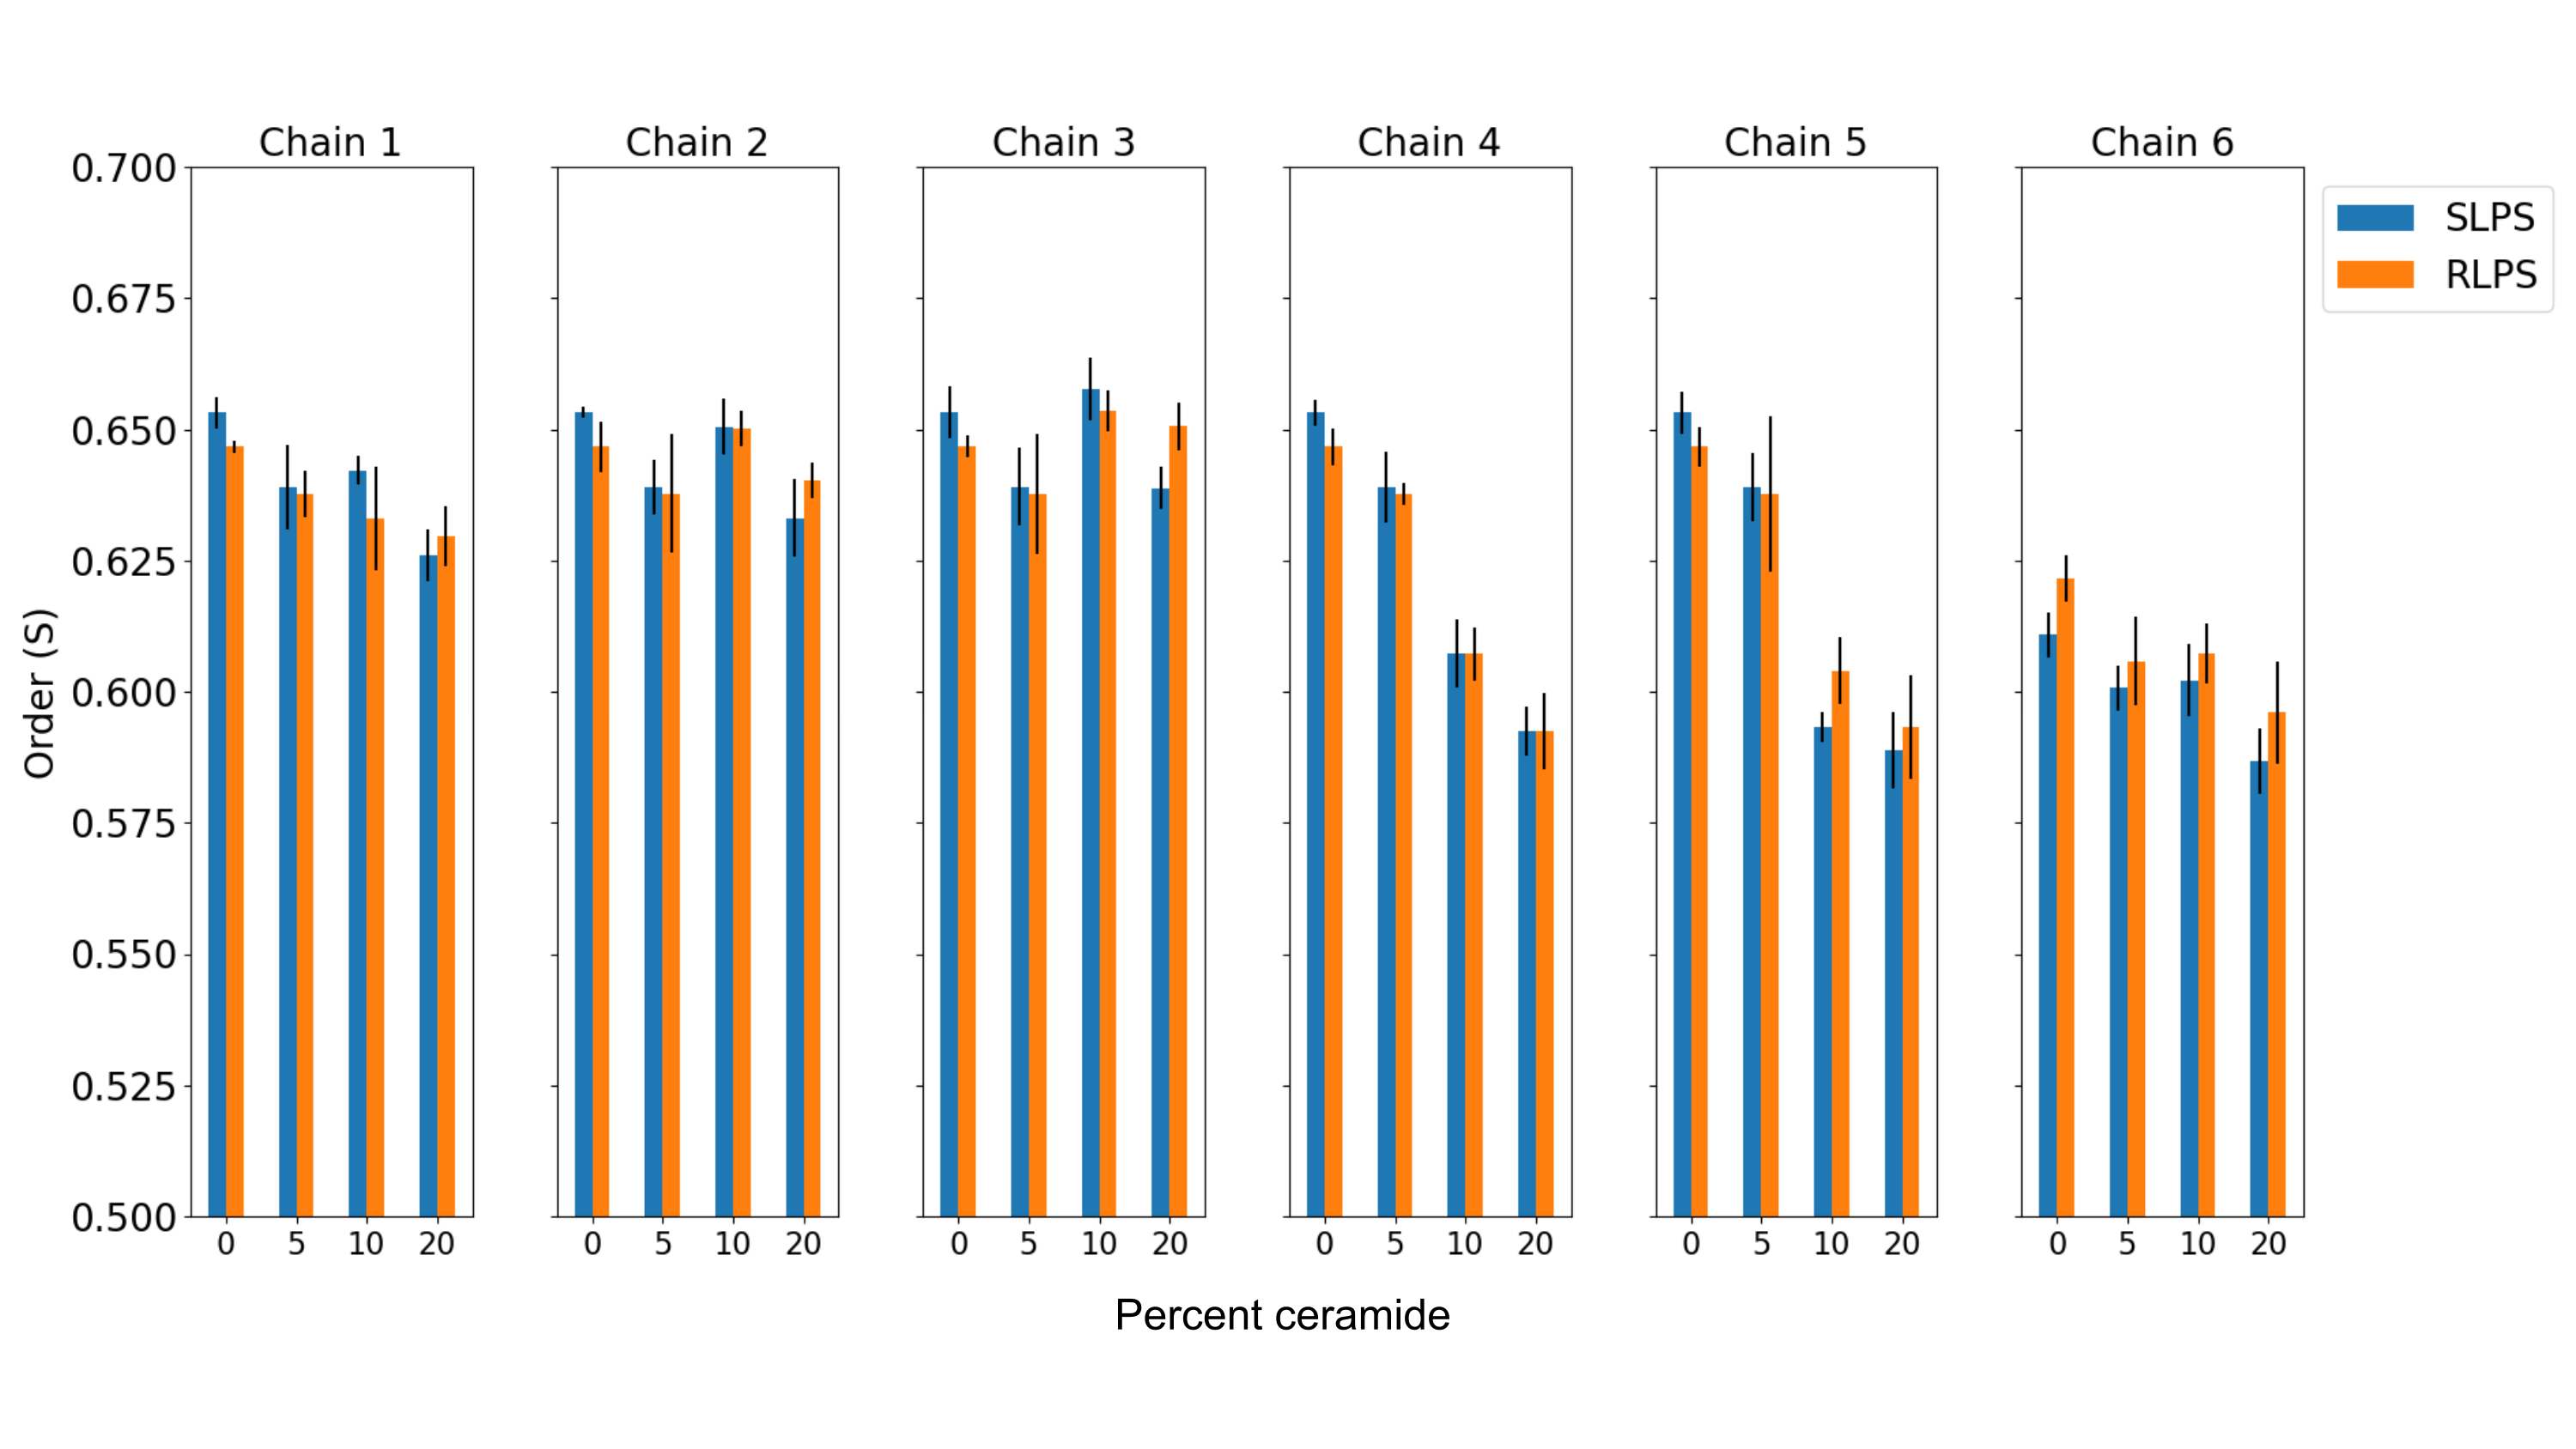
\includegraphics[width=13cm, scale=0.85]{MS thesis/figures/random_order_parameter.png}}
  \caption[Random Membrane: Order Parameter]{Random membrane: Order parameter of lipid A chains 1-6 of SLPS and RLPS. Lipid A acyl chains are numbered as shown in Figure \ref{fig:bond}. Order parameter calculated as described in the Methods. SLPS and RLPS are colored in blue and orange respectively. The error bars represent the standard error of three replicates per simulation. }
  \label{fig:ran_order}
\end{figure}

%% Random: Area per lipid and Peaks
Area per LPS was calculated by taking the X and Y dimensions of the system and dividing by the total number of LPS. 
The average area per LPS over the last \SI{5}{\micro\second}~of simulations did not show a significant difference between systems with 0\% and 5\% ceramide, with an average value of 3.7$\rm nm^2$. However, the area per LPS increased with increasing concentration of 10\% and 20\% ceramide (Figure \ref{fig:rand_apl}). 
As the LPS acyl chains become disordered, the chains expand further away from bilayer normal increasing the area per lipid, particularly in systems with higher ceramide concentrations. The increase in area with additional ceramide may indicate phase separation into liquid ordered and disordered ($\rm L_d$) phase.

%%% Random: area per lipid
\begin{figure}[H]
  \centerline{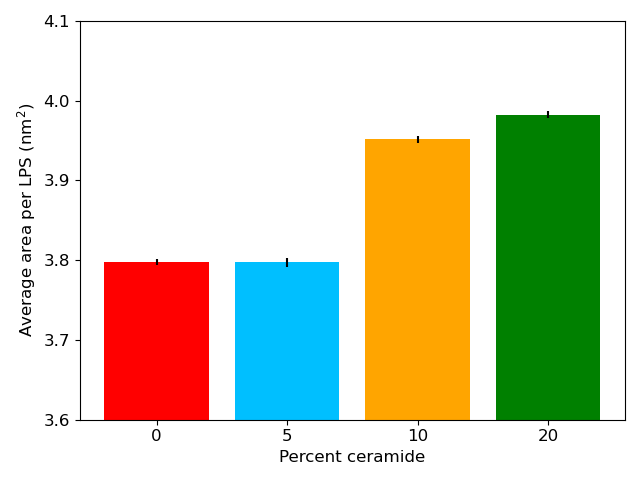
\includegraphics[width=8cm,scale=0.30]{MS thesis/figures/rand_apl_last_5us.png}}
  \caption[Random Membrane: Area per LPS]{Random membrane: Average area per LPS over the last \SI{5}{\micro\second} of simulation time. Area per LPS is the following for, 0\%, 10\%, 20\% ceramide:  3.80 $\pm$ 0.0038 $\rm nm^2$, 3.8$\pm$0.0056$\rm nm^2$, 3.9 $\pm$0.0043$\rm nm^2$, 3.9$\pm$0.004$\rm nm^2$, respectively. Area per LPS increased with increasing ceramide concentration. Error bars represent standard error across three replicates. }
  \label{fig:rand_apl}
\end{figure}

%% Random: Radial distributions
To further examine the interaction between SLPS and RLPS, radial distribution functions were measured. The radial distribution functions measure the probability of finding pairs of atoms at a distance of radius, r. Figure \ref{fig:rand_radial_dist}, demonstrates the radial distribution and the peak heights of the first three peaks, for the following pairs: RLPS-RLPS, SLPS-SLPS, SLPS-RLPS. In 0\% ceramide system, there was no peak found at 0.5nm radius. In 0\%, 5\%, and 10\% systems, there was a shift in RLPS-RLPS pair from peak 2 at 1.0nm to peak 3 at 1.35nm. RLPS molecules were more likely to be in proximity, before being \enquote{pushed} further away with the addition of 20\% ceramide (Figure \ref{fig:rand_radial_dist}A). Similarly for SLPS-SLPS pairs, in systems with 10\% ceramide, SLPS molecules were likely to be found close together at a radius of 1.5nm, due to the shift from peak 2 to peak 3. However, in systems containing 0, 5, and 20\%  concentration, the probability of finding SLPS near another SLPS decreased at 1.5nm (Figure \ref{fig:rand_radial_dist}B).
In a system with 0\% ceramide at a larger radius of 1.5nm, more SLPS and RLPS were closer to one another. At 0.5nm, more SLPS and RLPS were likely to be in proximity in the system with 10\% ceramide, but at 20\% concentration SLPS and RLPS were \enquote{pushed} apart from each other. (Figure \ref{fig:rand_radial_dist}C). At 10\% concentration LPS, pairs were likely to be found closer, however, increasing ceramide concentration further caused the pairs to be more spread apart.

 % Random: Radial distributions
 
\begin{figure}[H]
  \centering
  \subfloat{{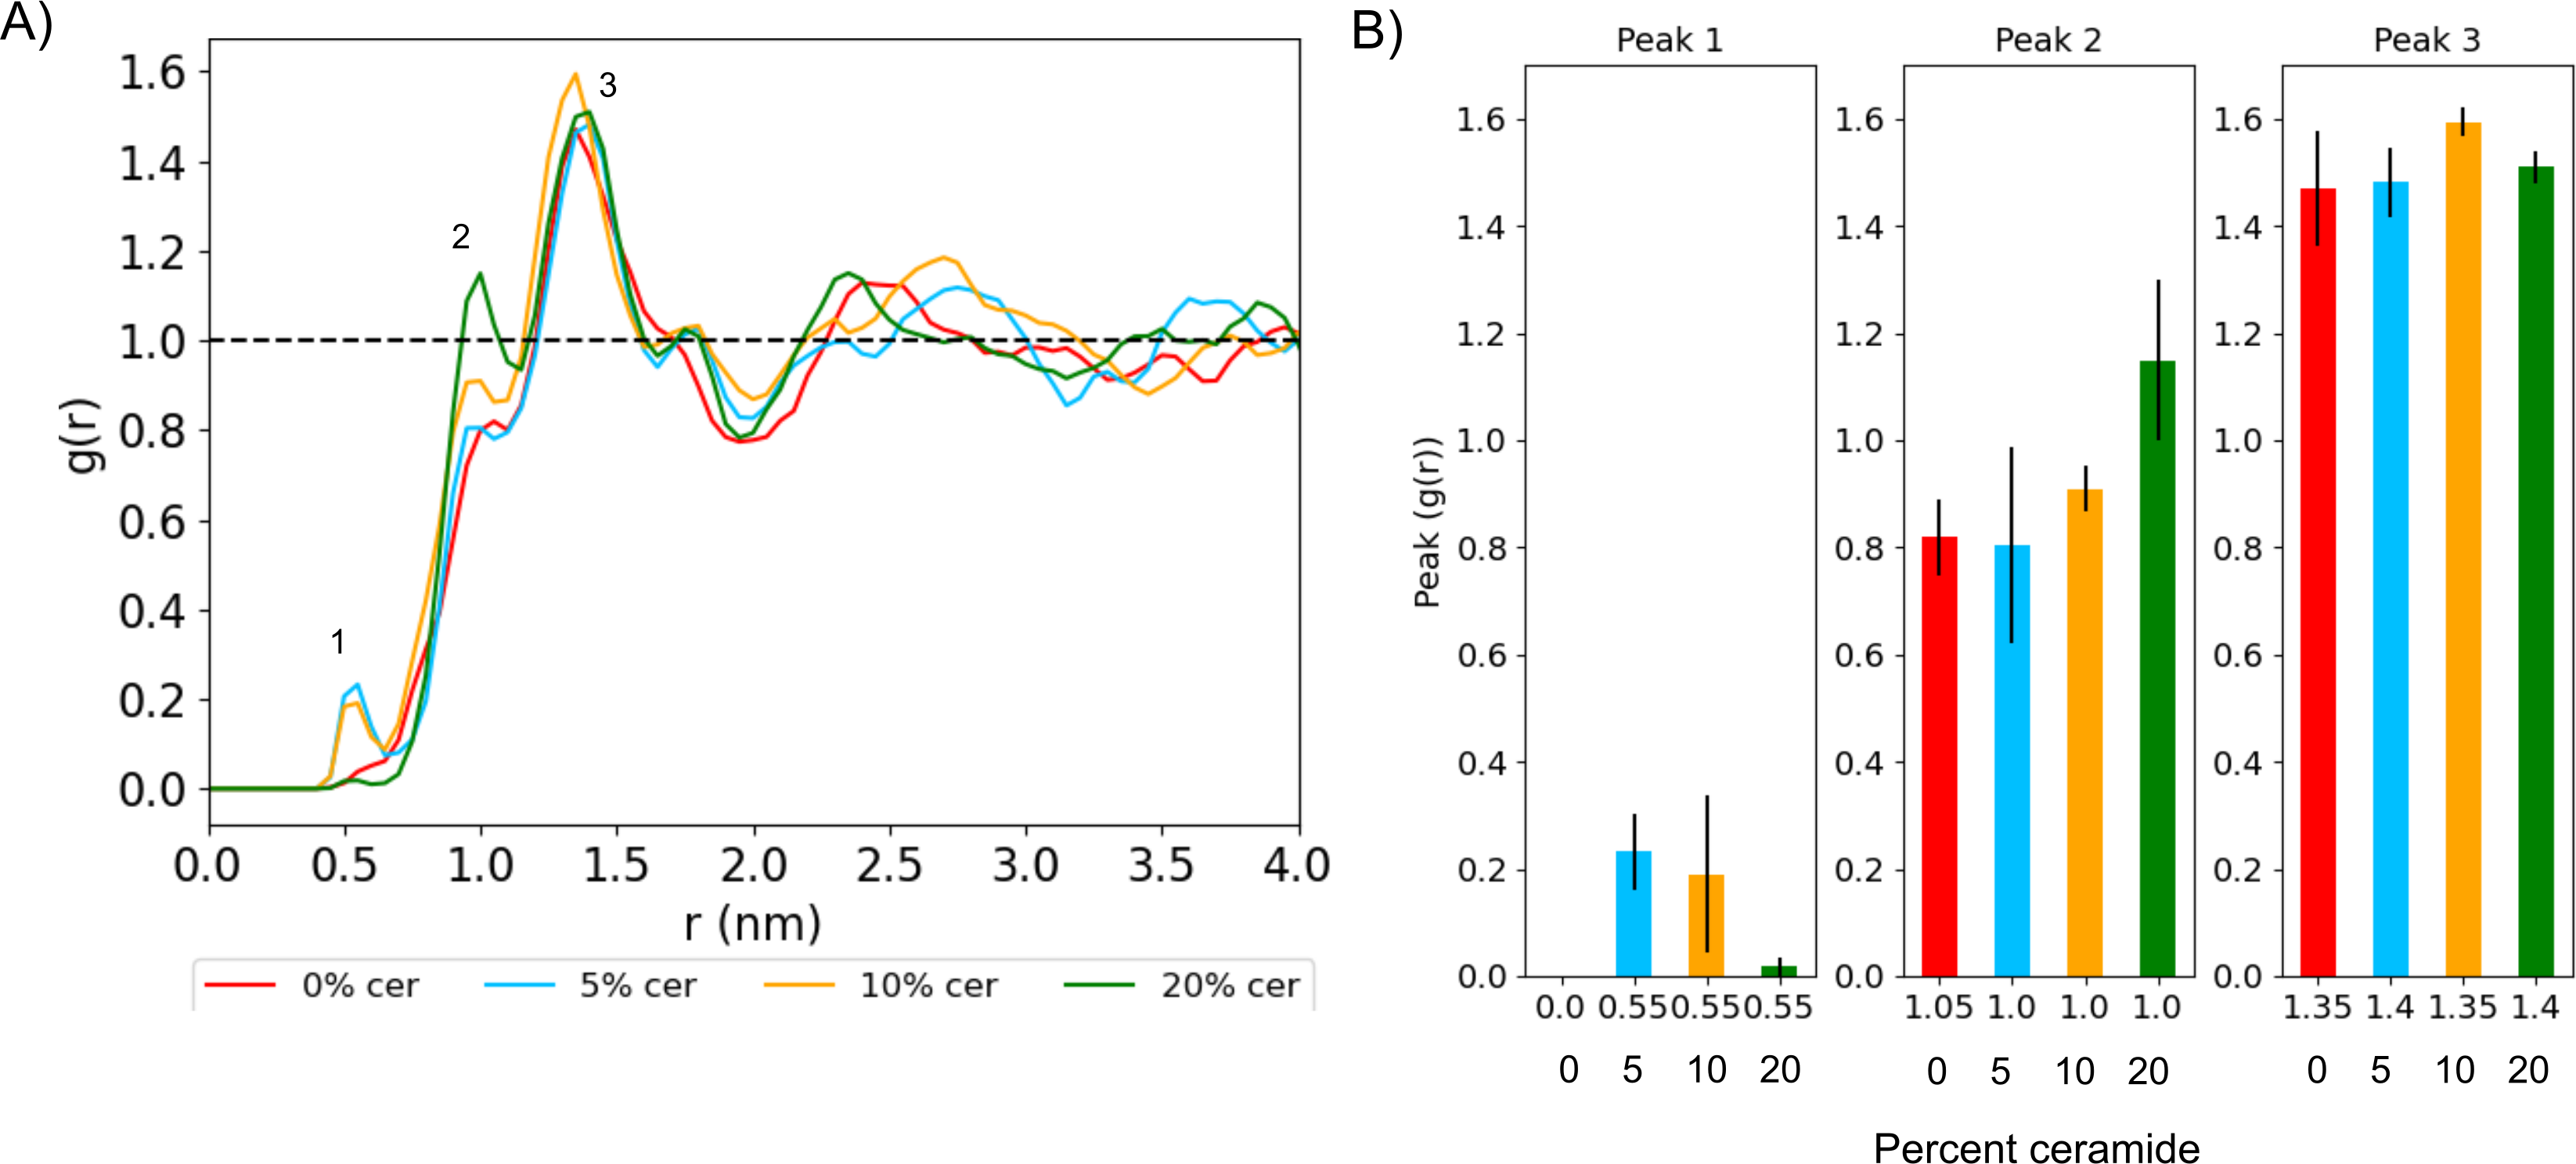
\includegraphics[width=12cm, scale=0.30]{MS thesis/figures/random_rdf_rough_rough_distribution_peaks-trim.png}}}
  \qquad
  \subfloat{{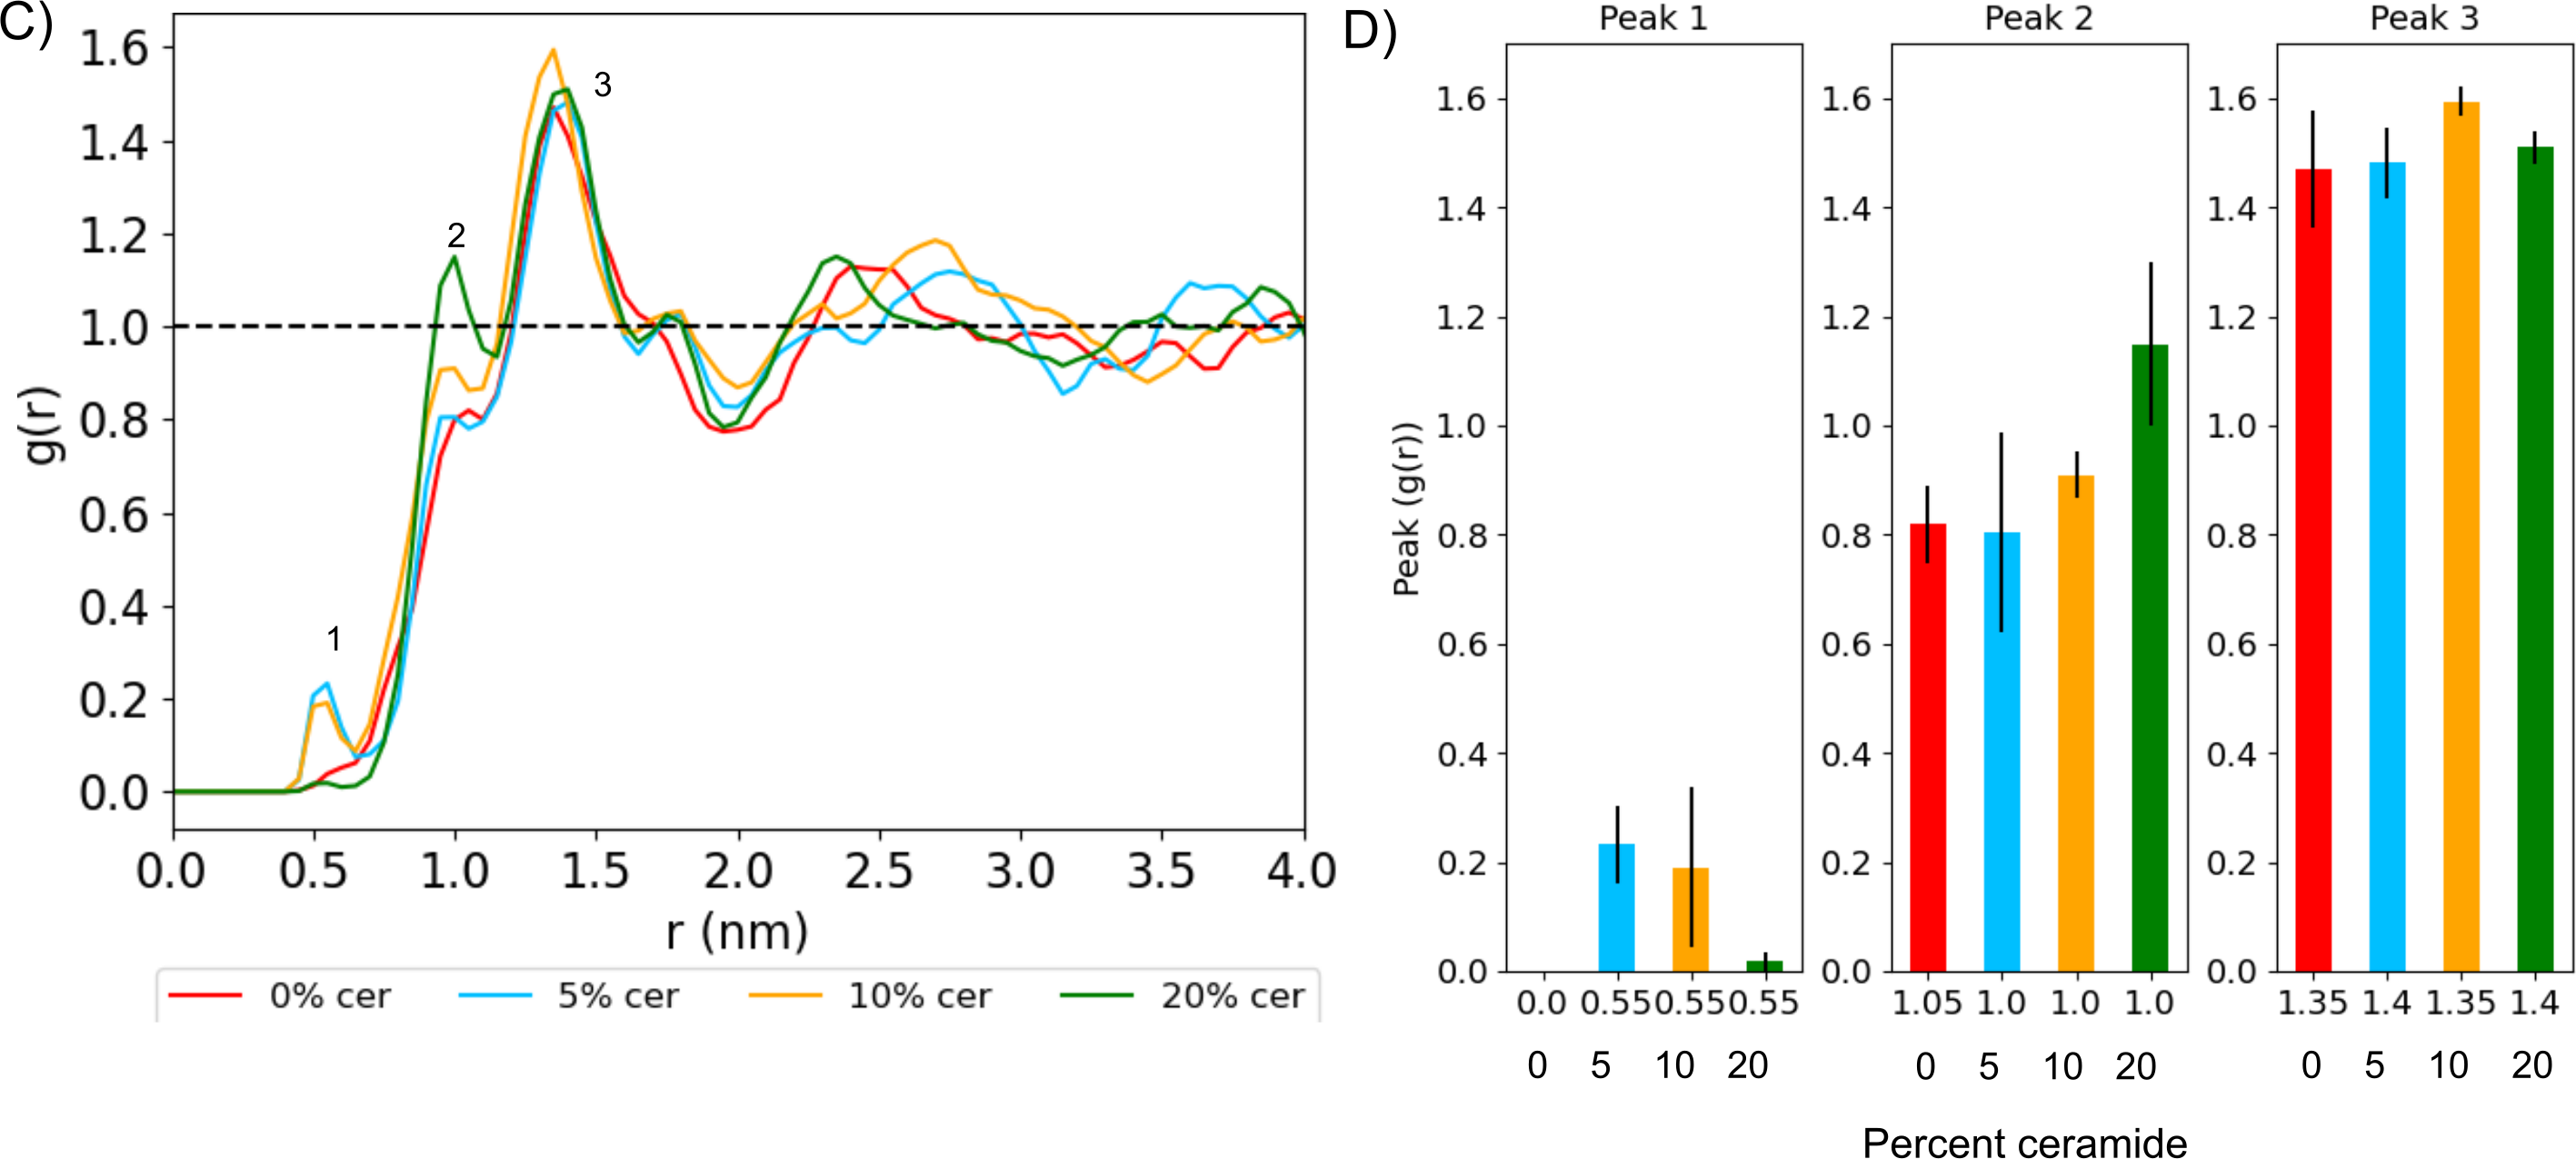
\includegraphics[width=12cm,scale=0.30]{MS thesis/figures/random_rdf_smooth_smooth_distribution_peaks-trim.png}}}
  \qquad
  \subfloat{{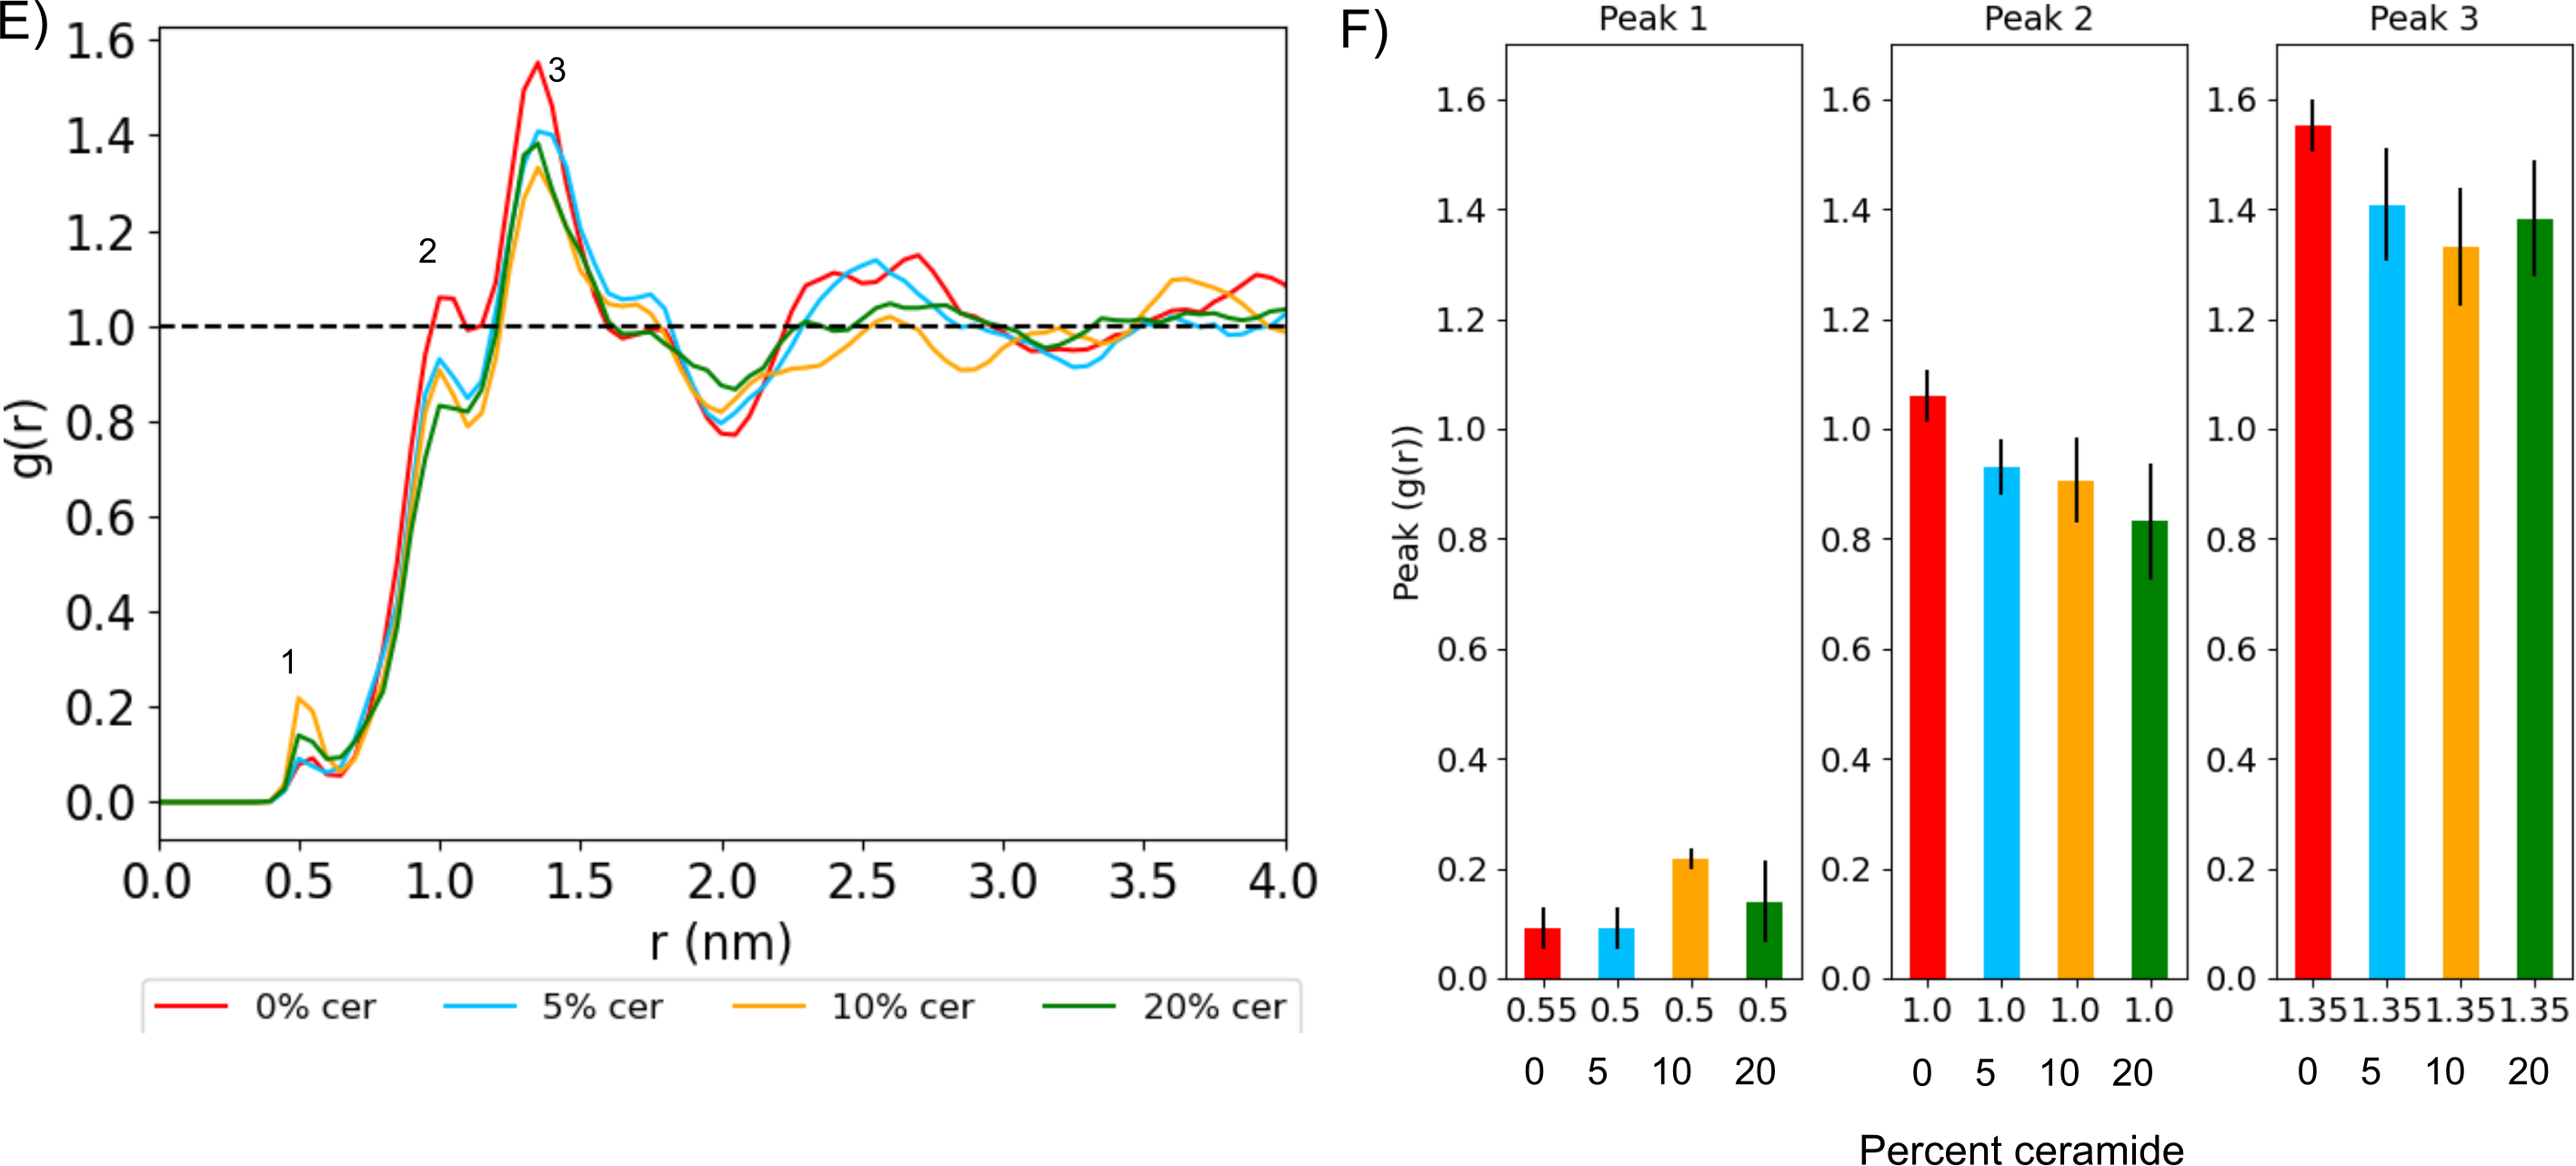
\includegraphics[width=12cm,scale=0.30]{MS thesis/figures/random_rdf_smooth_rough_distribution_peaks-trim.png}}}
  \caption[Random Membrane: Radial Distribution Function]{Random membrane: Radial distributions curve and the first three peaks heights. RLPS paired with respect to RLPS is on the top panel (A, B). (B) In system with 0\% ceramide, there was no first peak present at 0.5nm . SLPS paired with SLPS middle panel (C, D); SLPS paired with respect to RLPS bottom panel (E, F). The error bars represents standard error over three replicates. The first three peaks are labeled on the distribution curves(A, C, E). Plot color is as following: 0\% red, 5\% cyan, 10\% orange, 20\% green.}
  \label{fig:rand_radial_dist}
\end{figure}
\newpage
%% Random: Radius of gyration
We calculated the radius of gyration  over the last \SI{20}{\micro\second} in order to further understand lipid A mobility (Figure \ref{fig:ran_rgry}). A larger value of gyration suggests an increased deviation from the center of mass at each time point, from which we can confer about the acyl chain flexibility. SLPS in the system with 0\% ceramide showed an average value of 5.20\si{\angstrom^2}. The SLPS in the system with 20\% ceramide showed increased lipid A mobility with an average value of 5.32\si{\angstrom^2} (Figure \ref{fig:ran_rgry}A). There was no significant difference in the radius of gyration between 5\% and 10\% ceramide systems, for both the LPS variants. Furthermore, there is no difference in RLPS lipid A chain flexibility among the different ceramide concentrations (Figure \ref{fig:ran_rgry}B). 


\begin{figure}[H]
  \centering
  \subfloat{{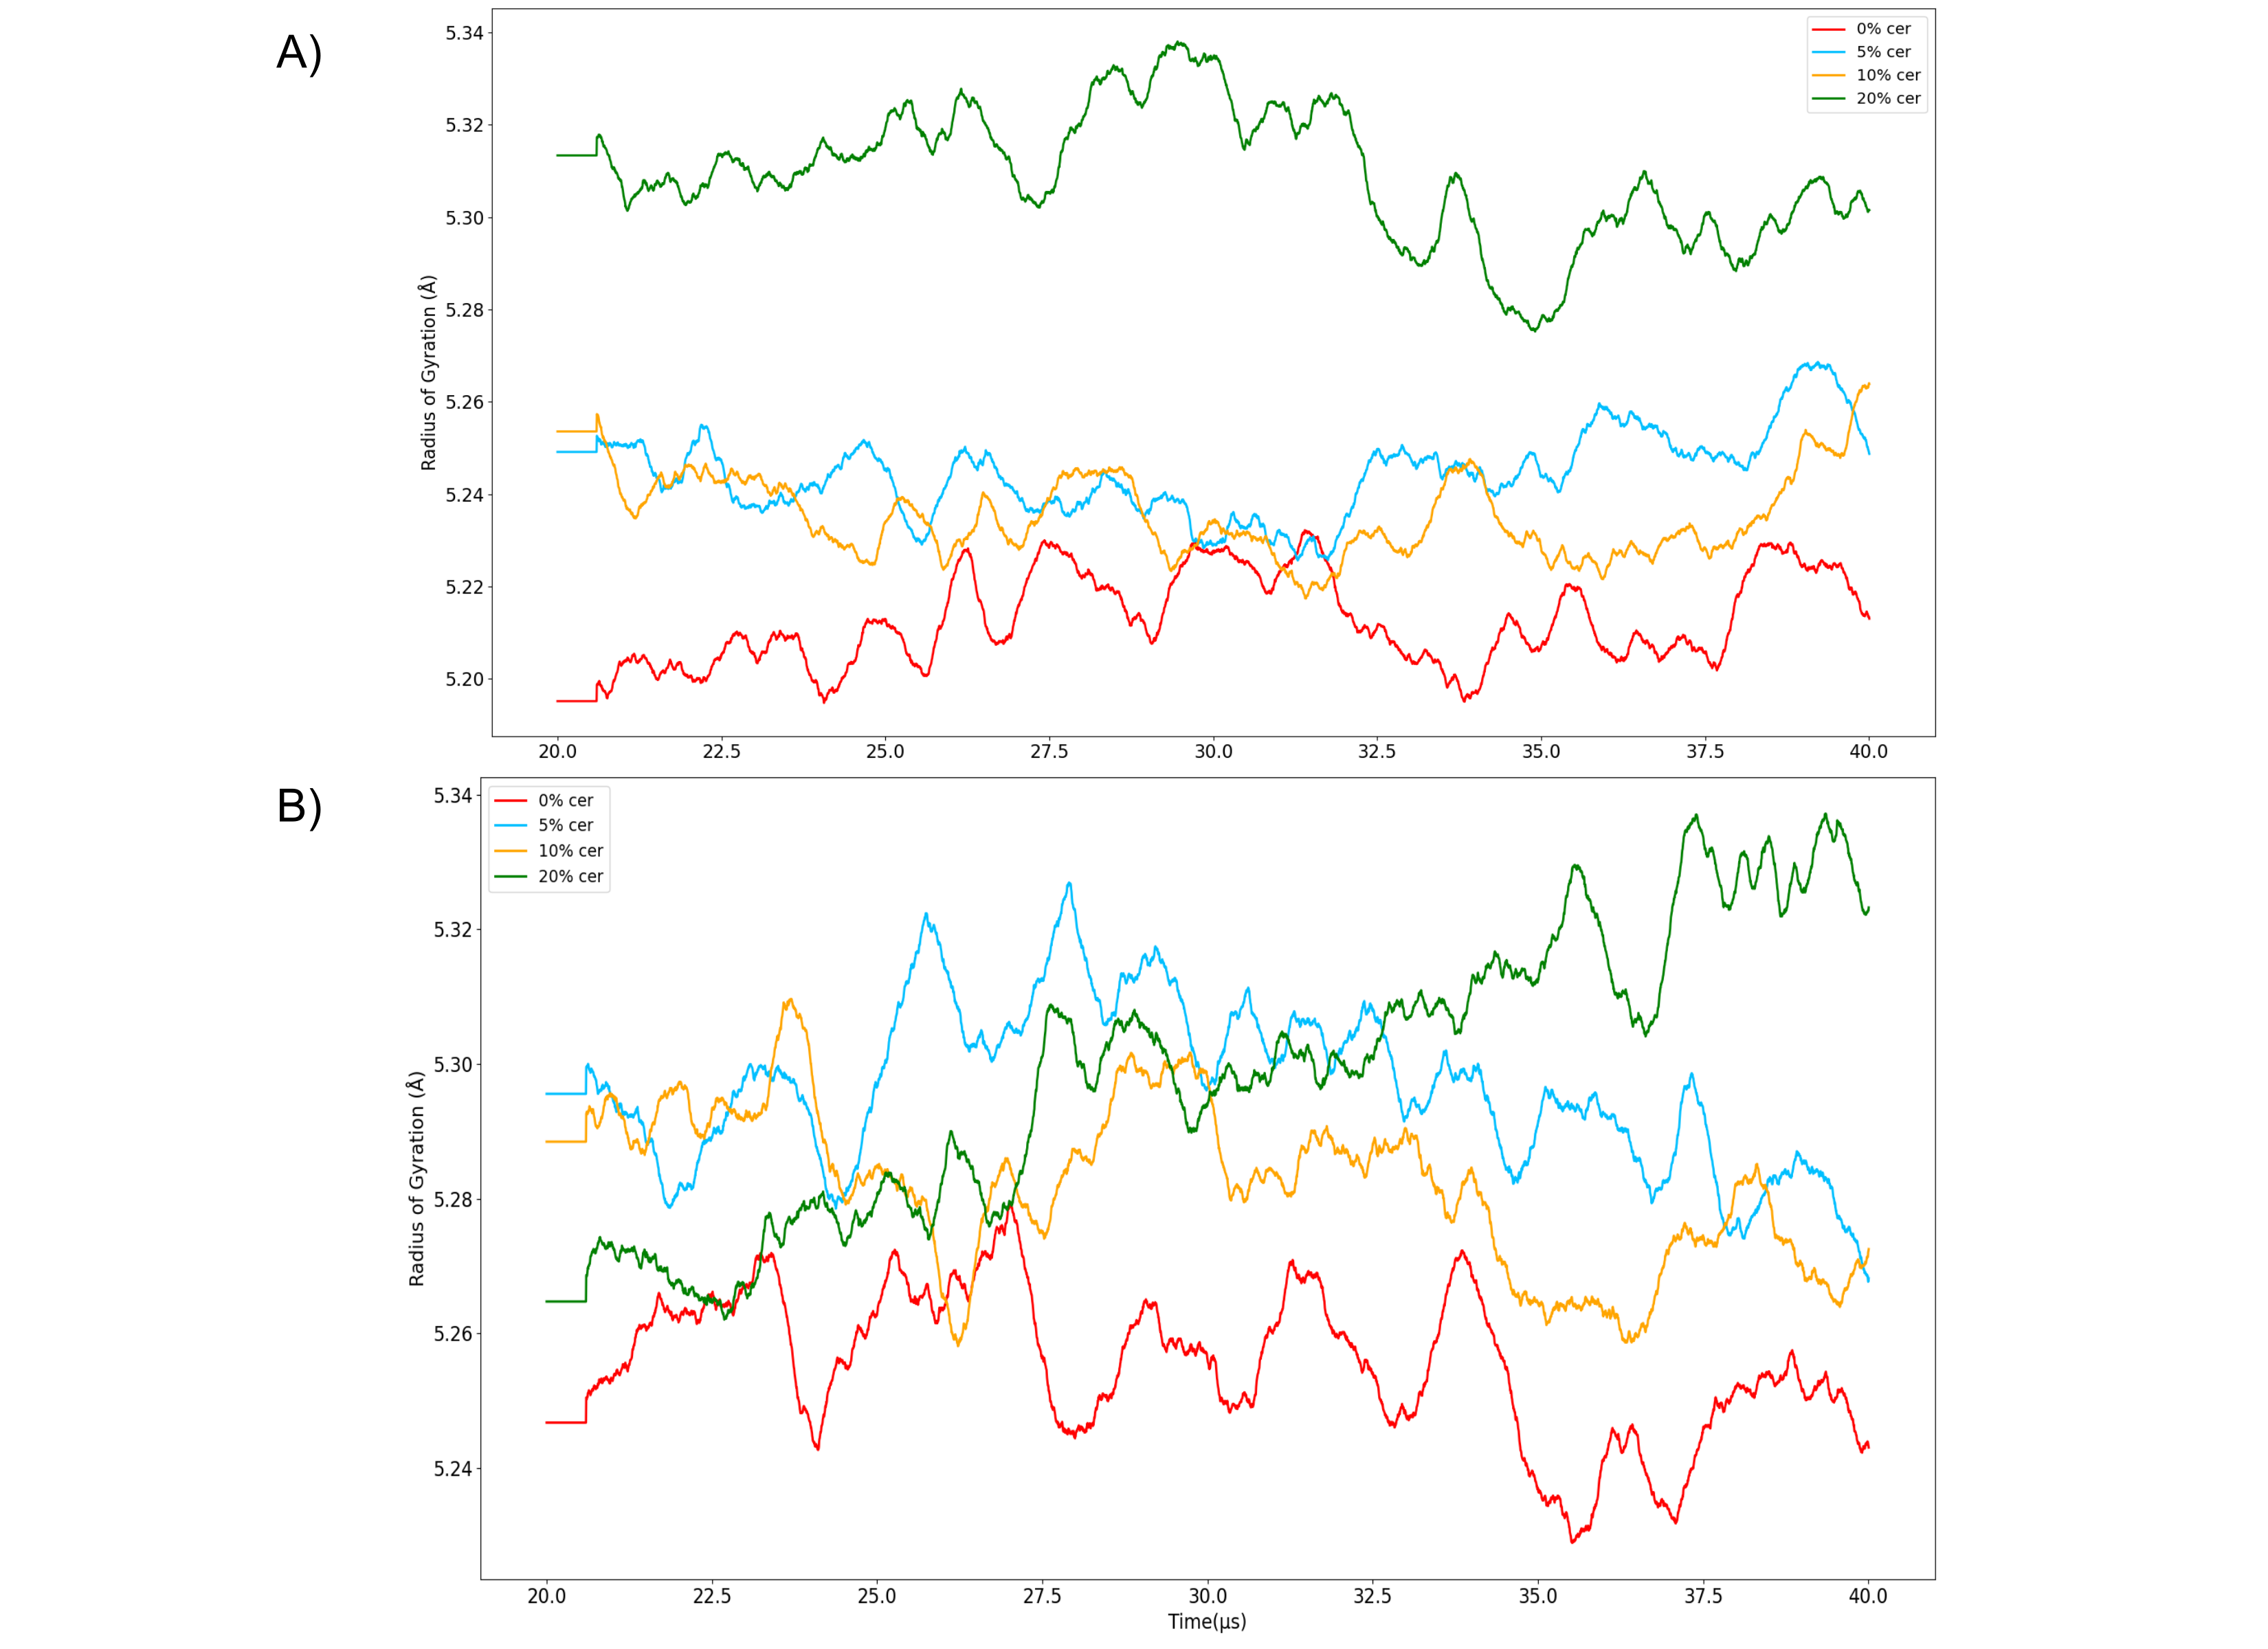
\includegraphics[width=\textwidth, scale=0.90]{MS thesis/figures/rand_rgyr_slps_rlps.png}}}
  \caption[Random Membrane: Radius of gyration]{Random membrane: Radius of gyration of lipid A over the last \SI{20}{\micro\second}.(A) SLPS radius of gyration. (B) RLPS radius of gyration. Radius of gyration was calculated as described in the Methods. Larger gyration values (y-axis) represent deviation from center of mass of lipid A, representing acyl chain mobility. Simulations with ceramide concentrations of 0\%, 5\%, 10\% and 20\% are colored in red, blue, orange and green curves respectively.
  }\label{fig:ran_rgry}
\end{figure}

\newpage
%% Bond Measurements
We measured interaction along the lipid A and ceramide acyl chains to examine whether ceramide and LPS had favorable interaction sites. We calculated the distance of each position of acyl chains in lipid A and ceramide for the last \SI{20}{\micro\second}; see figure \ref{fig:bond} for chain and bead position labels. Enrichment was calculated for pairs with a distance of 10\si{\angstrom} or less. For each interaction pair, the percentage was divided by the null hypothesis, where all pairs are equally likely to interact.  
Figure \ref{fig:rand_enrichment}, demonstrates the difference in enrichment between SLPS and RLPS along various sites of the acyl chains. Each grid in the heat map represents a pair of interactions between the corresponding ceramide position and a lipid A position. Acyl chains were numbered as shown in figure \ref{fig:bond}. 
In systems with 5\% and 20\% ceramide, RLPS lipid A sites were highly enriched as represented in red. In both 5\% and 20\% systems, lipid A acyl chain 1 shows the highest enrichment specifically close to sugar groups within the backbone. However, in the system with 10\% ceramide, there was a shift in enrichment towards SLPS, specifically for chains 1 through 3, possibly due to the repositioning of ceramide in the membrane. This may suggest a phase shift at 10\% ceramide concentrations, where the system is responding to the presence of ceramide differently. 



\begin{figure}[H]
%   \centerline{\includegraphics[width=\textwidth,scale=0.8]{MS thesis/figures/random_difference_enrichment-cropped.pdf}}
   \centerline{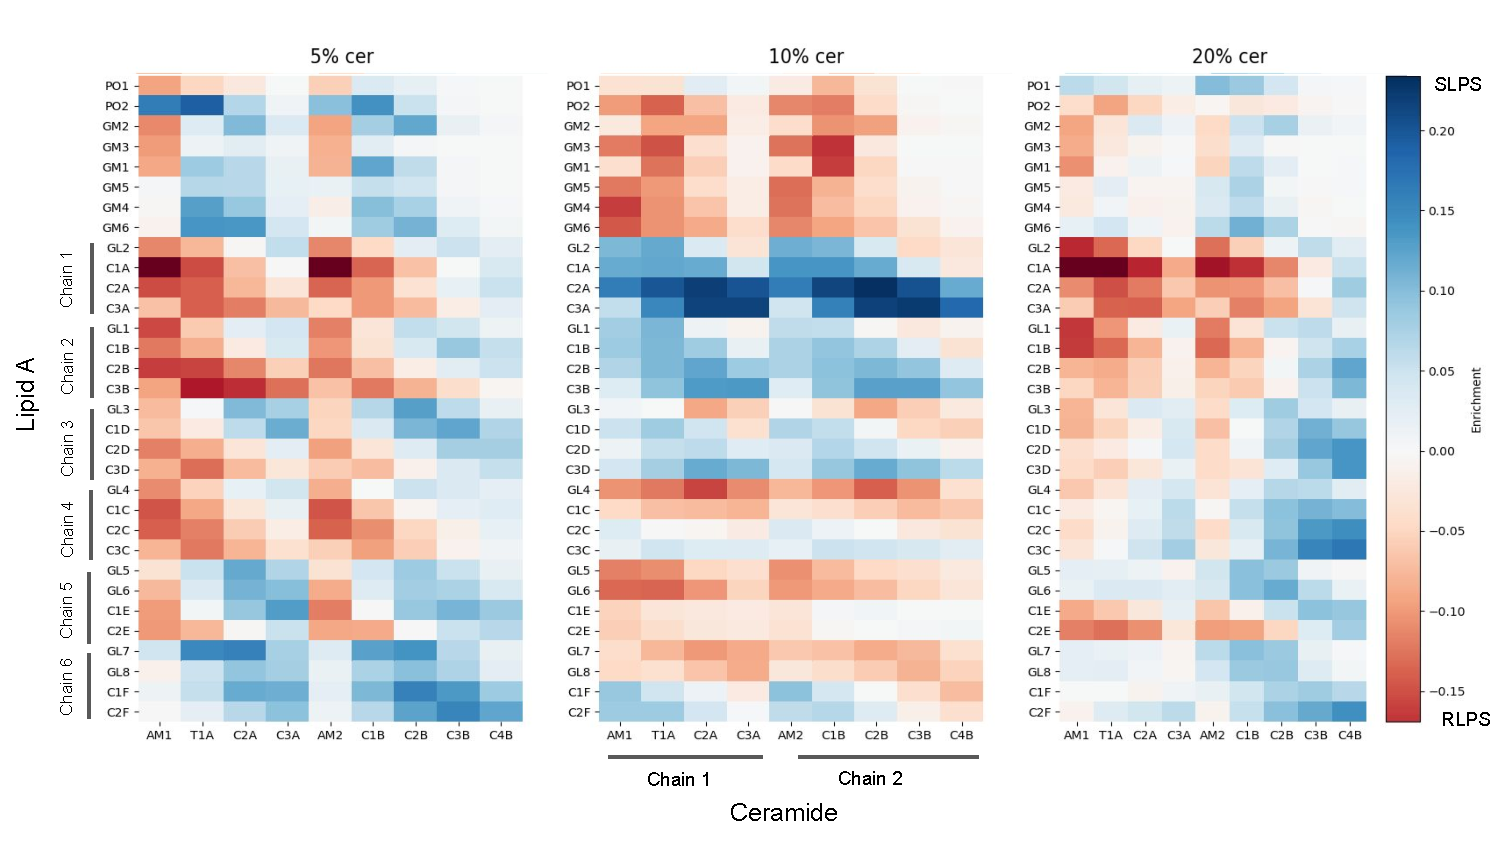
\includegraphics[width=\textwidth,scale=0.8]{MS thesis/figures/random_difference_enrichment.pdf}}
  \caption[Random Membrane: Ceramide Enrichment]{Random membrane: Heat map of difference in enrichment between SLPS and RLPS. Axes represent the location along acyl chains; ceramide on the x-axis and LPS lipid A on the y-axis. The chain positions are labeled according to Martini nomenclature. The chain number is as labeled in figure \ref{fig:bond}. Blue color represents higher enrichment in SLPS, and the red color represents high enrichment in RLPS.}
  \label{fig:rand_enrichment}
\end{figure}

\newpage
 
%% Artificial membrane
\subsection{Artificial Membrane}
\par We built an artificial membrane containing an island of SLPS, surrounded by a larger region of RLPS, to further understand the effect of ceramide along separated regions of SLPS and RLPS, as well as the interface between the two LPS lipids types (Figure \ref{fig:intro}).
The composition of the outer leaflet of the membrane contained a 1:3 ratio of SLPS to RLPS. Three replicates of the five simulations containing ceramide concentrations of  0\%, 10\%, 15\%, 20\%, and 25\% were performed. 

We calculated the order parameter for the artificial membranes, in the same manner as the randomized membrane, see figure \ref{fig:art_order}. Chain 1 of SLPS showed an increase in order as ceramide concentration increased. For SLPS acyl chains 2 and 3, the order increased from 10\% ceramide to 15\% ceramide system.
RLPS orders decreased in the system with 20\% and 25\% ceramide, across chains 1 through 3. Similar to the randomized membrane, the artificial membrane showed more disorder in chains 4 through 6 of both  RLPS and SLPS. Within the artificial membrane, RLPS lipid A was more ordered as compared to SLPS lipid A across the five different ceramide concentrations. 


%% Artificial membrane: chain order
\begin{figure}[H]
  \centerline{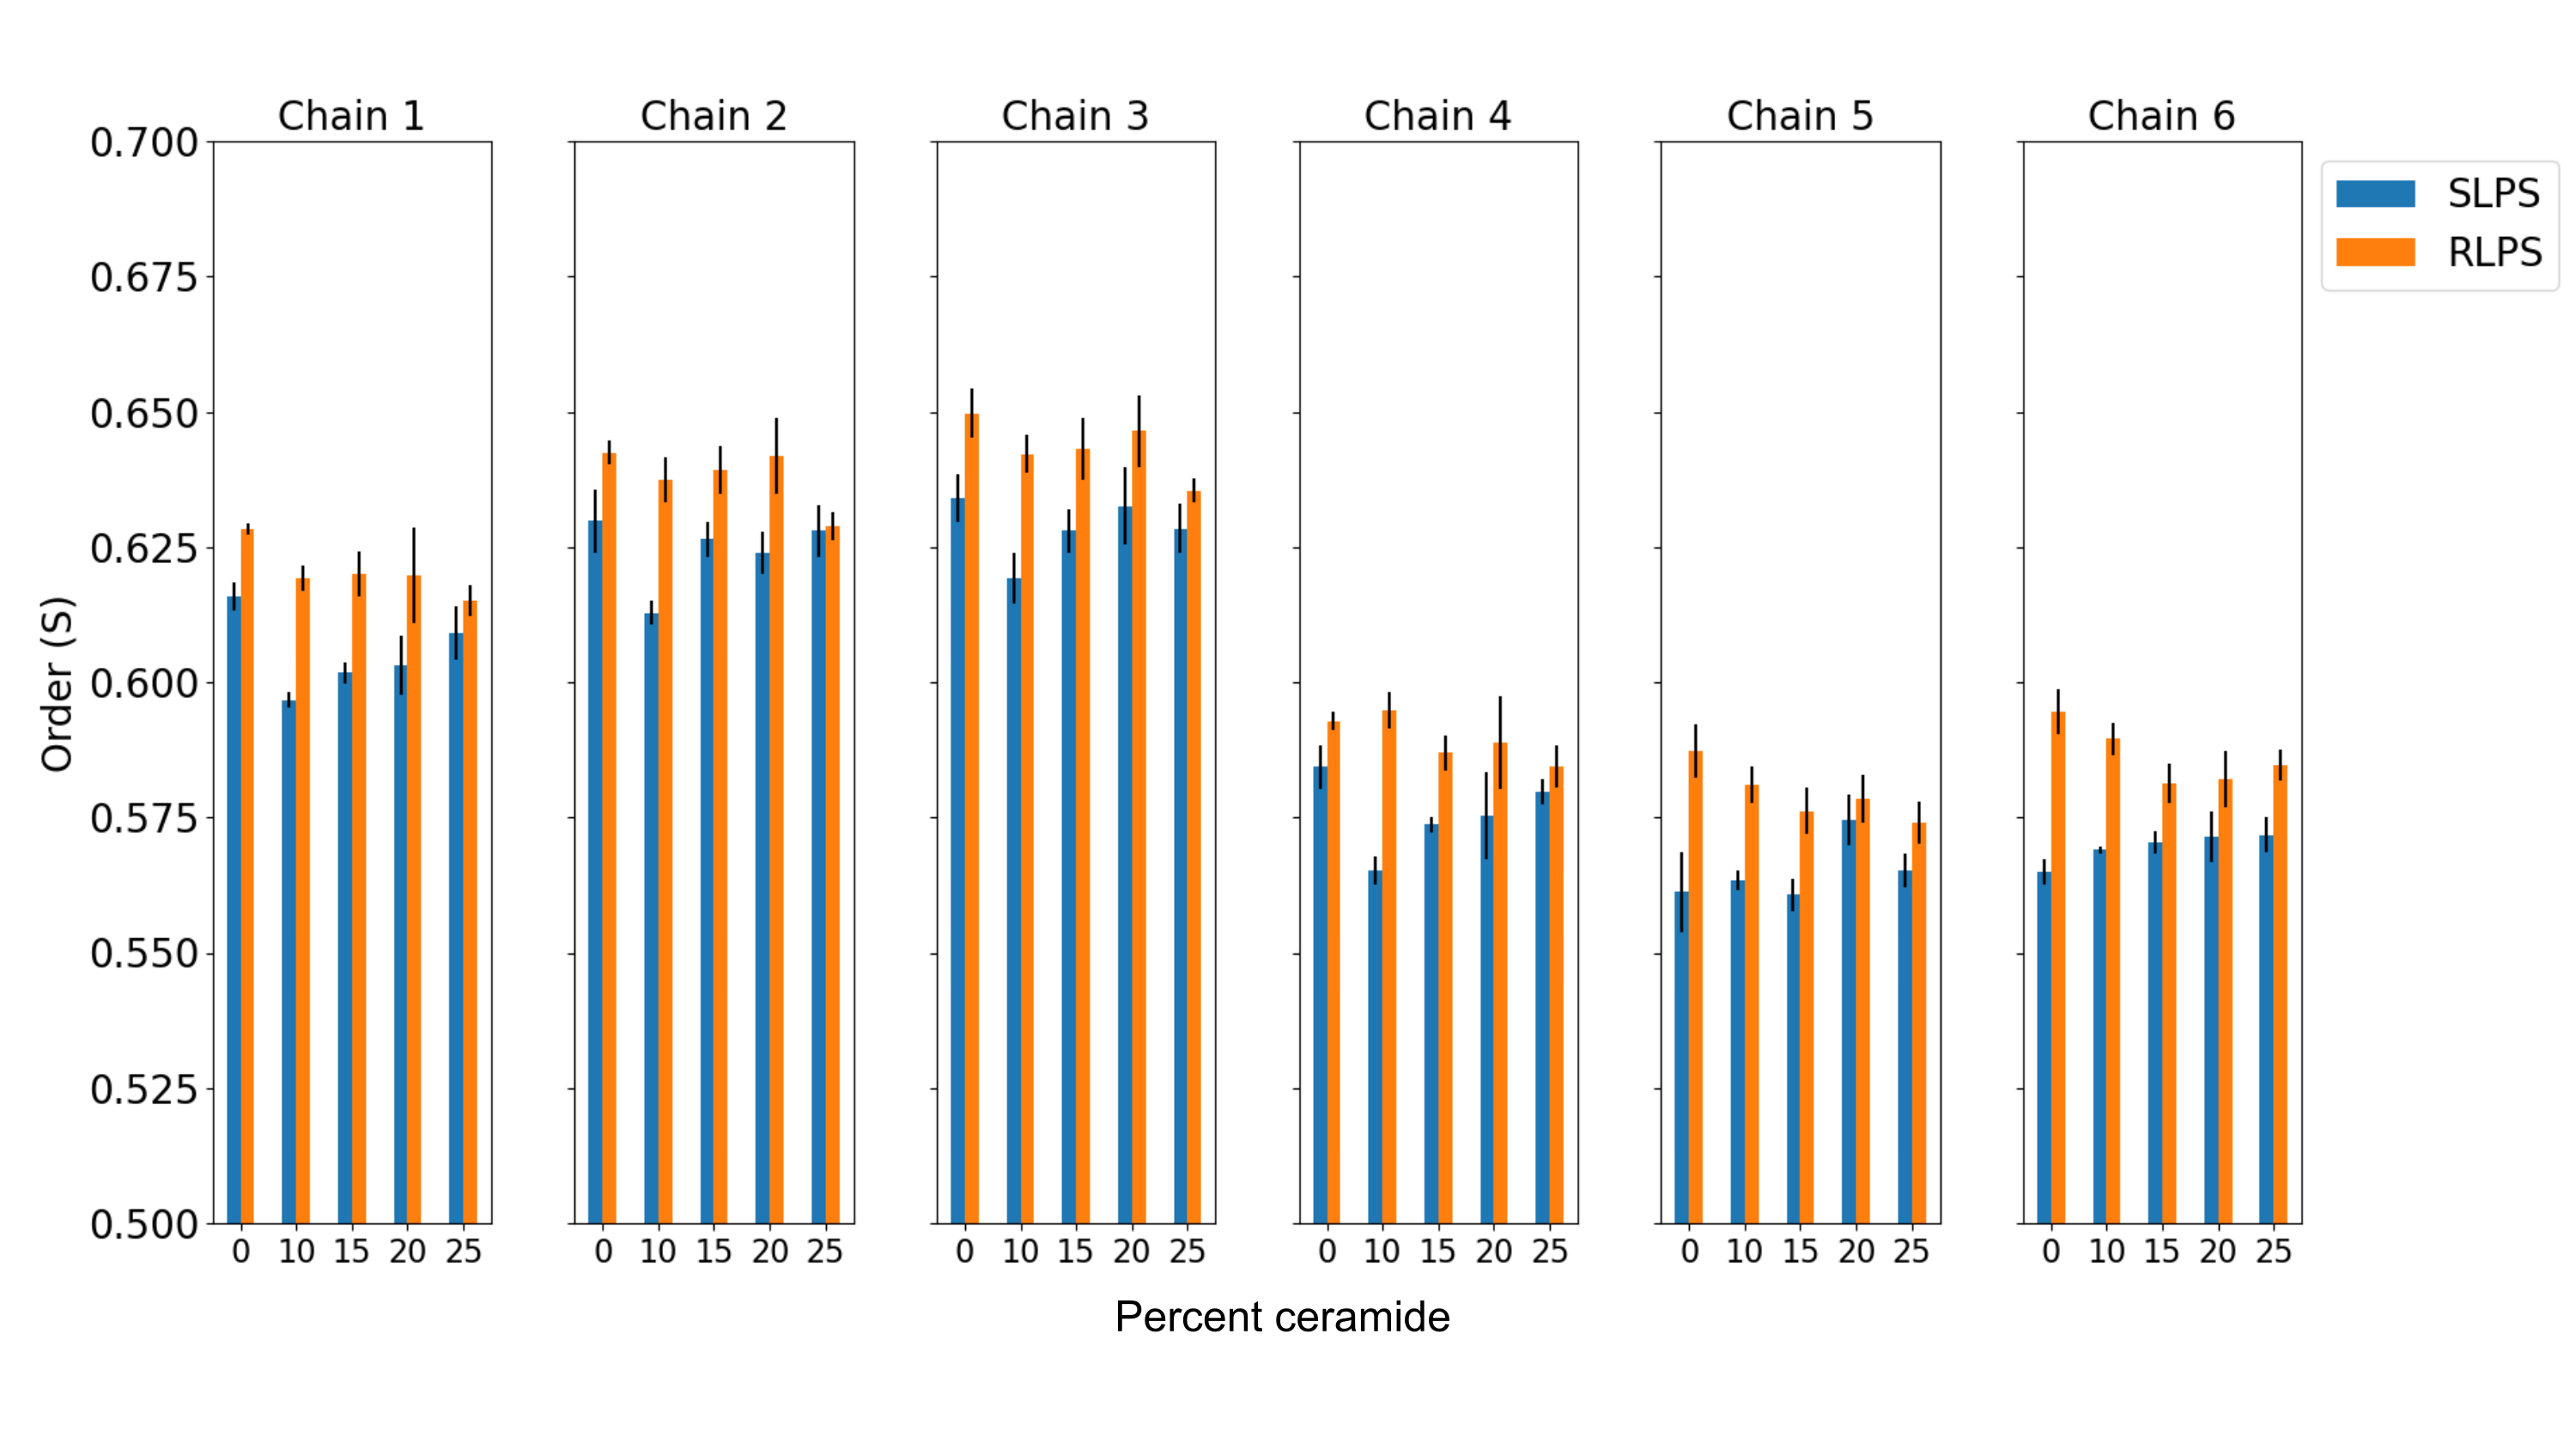
\includegraphics[width=15cm, scale=0.4]{MS thesis/figures/artifical_order_parameter.png}}
  \caption[Artificial Membrane: Order Parameter]{Artificial Membrane: Order Parameter of chains 1-6 of SLPS and RLPS across the five ceramide concentration. SLPS and RLPS are colored in blue and orange respectively. Lipid A acyl chains are numbered as show in in figure \ref{fig:bond}. Error bars represent standard error over three replicates.}\label{fig:art_order}
\end{figure}
\newpage
Area per LPS increased in the system of 0\% to 15\% ceramide with average values of 1.8$\rm nm^2$~to 2.1$\rm nm^2$~respectively. At 20\% ceramide concentration, relative area per LPS decreased to 2.0$\rm nm^2$. Interestingly, there was not a significant change in the area in the system with 25\% as compared to 20\% ceramide system (Figure \ref{fig:art_apl}). Taken together with the order parameter, this corresponds to lipid characteristics found in the liquid ordered and disordered phases, which might suggest that RLPS and SLPS had separated into two separate domains.

\begin{figure}[H]
  \centerline{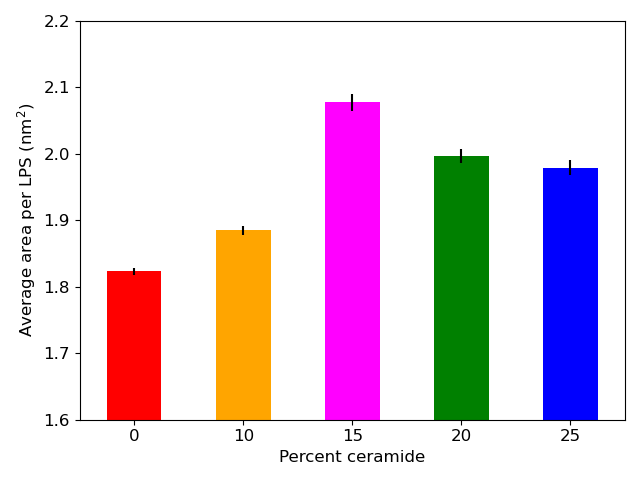
\includegraphics[width=10cm,scale=0.35]{MS thesis/figures/artificial_membrane_apl_last_5us.png}}
  \caption[Artificial Membrane: Area per LPS]{Artificial membrane: Average area per LPS over the last \SI{5}{\micro\second}~of simulations. Area for, 0\%, 10\%, 15\%,20\% and 25\% ceramide is the following:1.82 $\pm$ 0.0055$\rm nm^2$, 1.88 $\pm$0.0067$\rm nm^2$, 2.08 $\pm$0.013$\rm nm^2$, 1.99$\pm$0.010$\rm nm^2$, 1.97$\pm$0.011$\rm nm^2$ respectively. Area per LPS increased until 15\%, before decreasing at 20\% and 25\% ceramide. Error bars represent standard error, (n=3).}\label{fig:art_apl}
\end{figure}


%%%Artificial membrane: Radial Distributions

We investigated the interactions between each of the LPS variants using the radial distribution function (rdf). The radial distribution curves show the probability of finding pair of atoms within a given radius, r. The rdf was calculated for the following pairs: RLPS-RLPS and SLPS-SLPS across the five ceramide concentrations. SLPS-RLPS interaction was omitted as the two LPS types are separated into distinct regions. 
From the distribution plots, we located the first three peaks, labeled 1-3 in the distribution curves (Figure \ref{fig:art_radial_dist}). The peak height for the first three peaks is plotted alongside the distribution curves for each calculated pair. Figure \ref{fig:art_radial_dist}A, represents the reference distribution of 0\% ceramide, RLPS-RLPS and SLPS-SLPS pairs. For the RLPS-RLPS pairs, (Figure \ref{fig:art_radial_dist}B,C), the pair shifted from peak 2 at 1.0nm to peak 3 at 1.35nm across the ceramide concentrations. RLPS lipids were moving out of peak 2 to peak 3, suggesting RLPS-RLPS pairs were likely to be found closer together at a larger radius. In the 0\% system, SLPS shifted from peak 2 at 1.0$\rm nm$ to peak 3 at 1.4$\rm nm$ (Figure \ref{fig:art_radial_dist}D, E). SLPS in 15\% ceramide system showed a larger shift from peak 2 toward peak 3. At peak 3, more SLPS in the system with 0\% and 15\% were likely to be found closer together. Increasing ceramide concentration to 20\% and 25\% showed a decrease in peak 3 amplitude. SLPS lipids were pushed further away from other SLPS with increasing ceramide concentrations.


%%Artificial membrane: Radial distribution
\begin{figure}[H]
  \centering
  \subfloat{{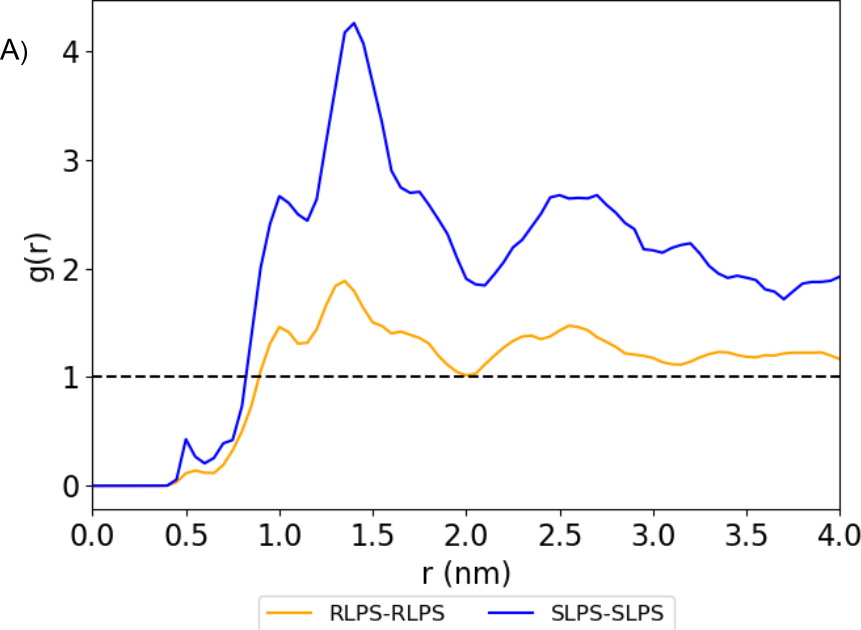
\includegraphics[width=8cm,  scale=0.80]{MS thesis/figures/artificial_rdf_distribution_nocer_rr_ss-trim.png}}}
  \qquad
  \subfloat{{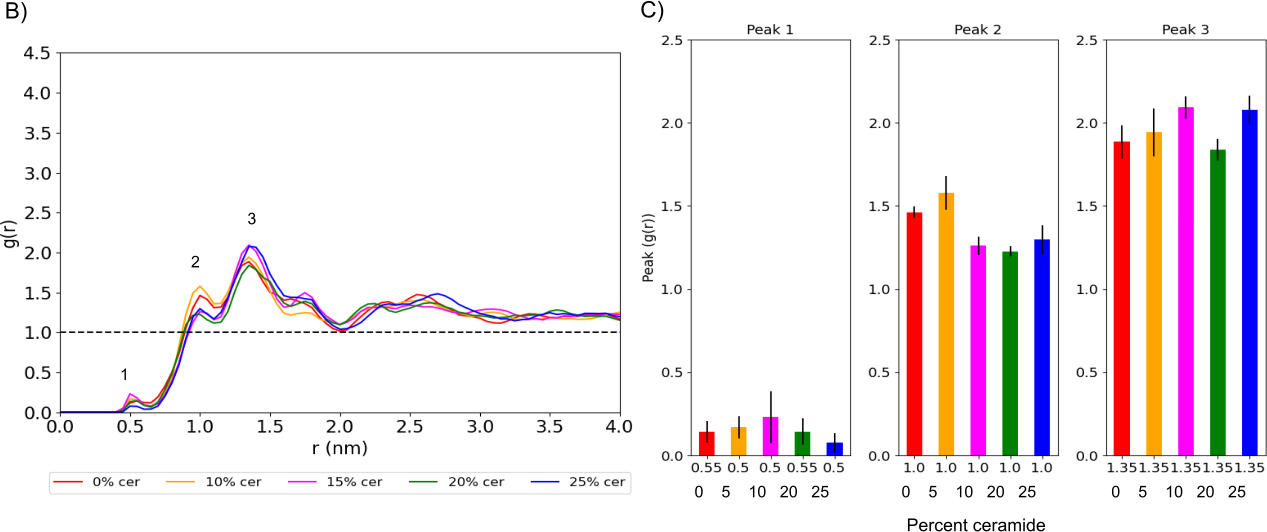
\includegraphics[width=15cm, scale =0.95]{MS thesis/figures/artificial_rdf_distribution_peak_rough_rough-trim.png}}}
  \qquad
    \subfloat{{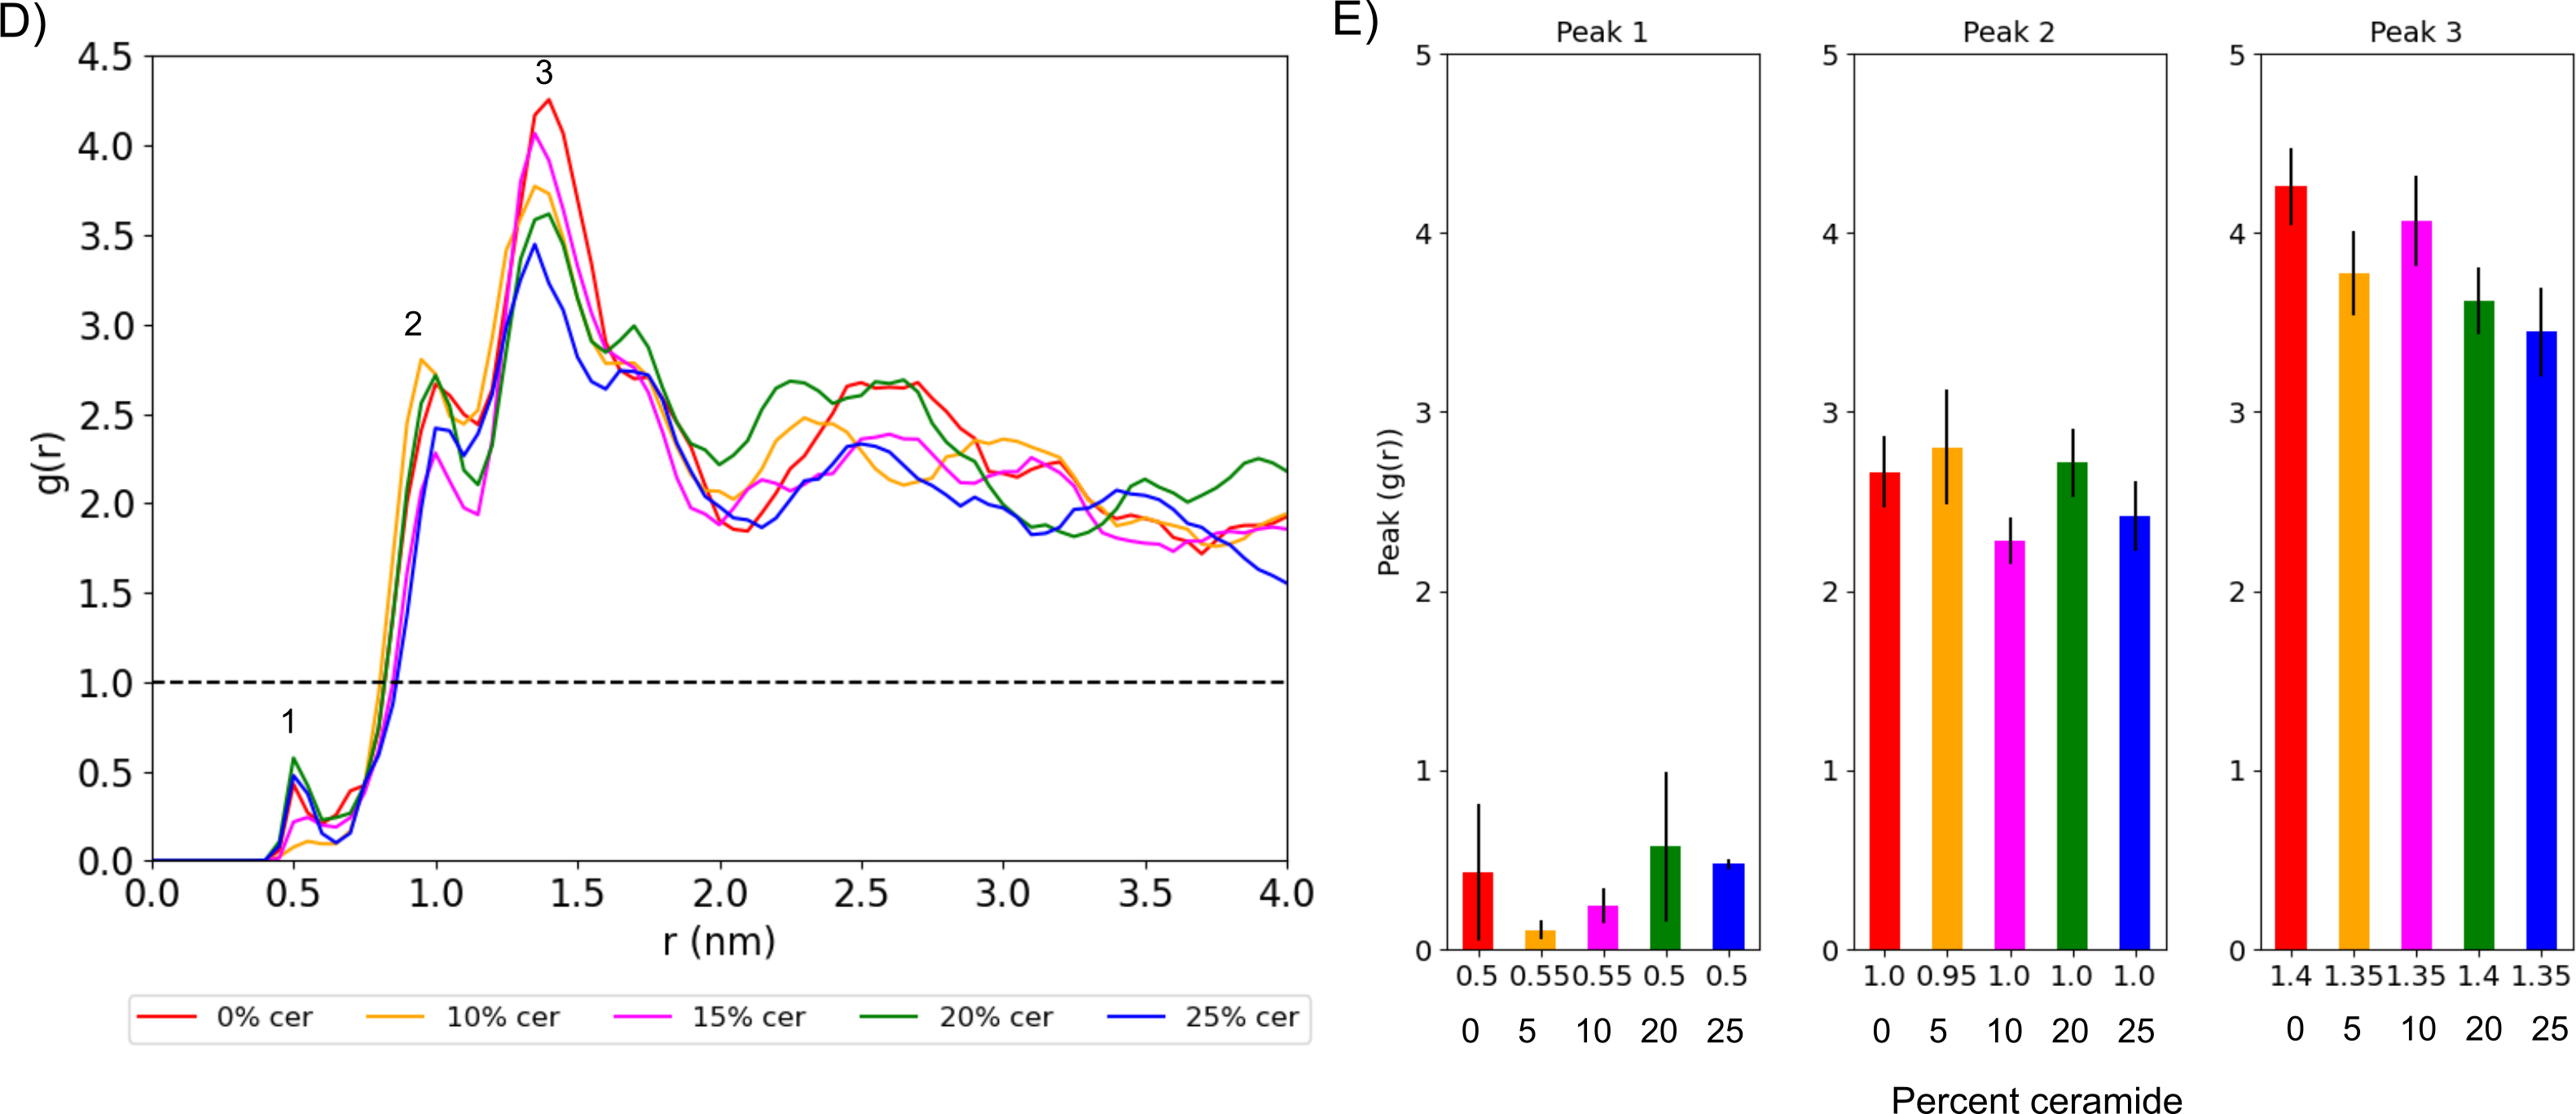
\includegraphics[width=15cm, scale =0.95]{MS thesis/figures/artificial_rdf_distribution_peak_smooth_smooth-trim.png}}}
  \caption[Artificial Membrane: Radial Distribution Function]{Artificial membrane: Radial distributions and the first three peak heights. (A) 0\% ceramide rdf as reference distribution. Blue represents SLPS paired with SLPS, orange curve represents RLPS paired with RLPS. 
  (B)radial distribution curves of RLPS paired with RLPS. (C) First three peak height and position of RLPS-RLPS pair as labeled in B. (D) Radial distribution curves of SLPS paired with SLPS. (E) The first three peak heights and positions, labeled in D. The error bars on the bar chart represent a standard error (n=3). The color scheme is the following: 0\% red, 10\% orange, 20\% green, 25\% blue.
  }\label{fig:art_radial_dist}
\end{figure}


Based on our visual observation of ceramide density in the artificial membrane, we hypothesized that ceramide may have a preference for occupying the boundary region between RLPS and SLPS. We investigated this by quantifying ceramide occupancy at three different regions within the simulation box: the RLPS region, the SLPS region, and the interface of RLPS and SLPS, as shown in figure \ref{fig:number_cer}A. A distance of 4.7\si{\angstrom} was set as the maximum radius between LPS and ceramide molecules. Selections were made such that ceramide could only be in one of the three regions, with no overlaps at a given time point. Ceramide enrichment was calculated by taking the percent of ceramide within each of the three regions and dividing by the number of LPS in each domain. Across ceramide concentrations, ceramide was highly enriched in the SLPS region in contrast to the RLPS and the boundary region, particularly.
As the concentration of ceramide increased, fewer ceramides were found within the boundary region (Figure \ref{fig:number_cer}B). 


Due to the slow diffusion of LPS, we were unable to observe domain formation within the simulation time. However, we were able to examine several characteristics of lipids typically found within the distinct domains. For both the artificial and the random membranes, the area per LPS increased with increasing ceramide concentration, with the largest area found in 15\% ceramide. Additionally, the order parameters showed similar trends in both systems, RLPS was more ordered while SLPS was more disordered. This may suggest phase separation of RLPS into liquid ordered phase and SLPS into liquid disordered phase.  


%% Artificial membrane: ceramide occupancy
 \begin{figure}[H]
  \centering
  \subfloat{{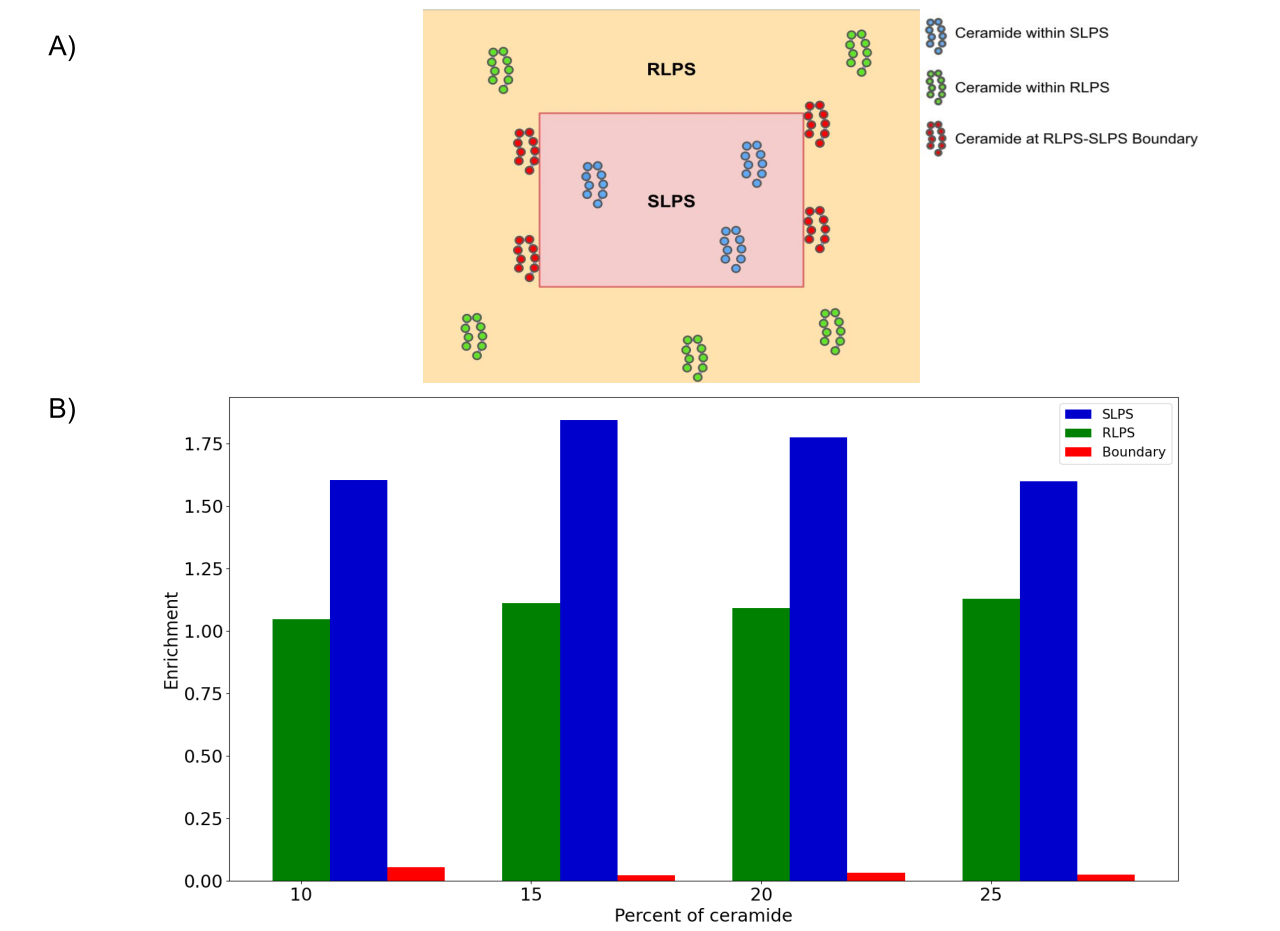
\includegraphics[width=13cm,scale=0.75]{MS thesis/figures/artificial_ceramide_enrichment.png}}}
  \caption[Artificial membrane: Ceramide Occupancy]{Artificial membrane: Ceramide occupancy in three regions of the simulation box, RLPS, SLPS, and RLPS-SLPS boundary. (A) Cartoon representing ceramide occupancy calculation method. Blue ceramides positioned within the inner box are in SLPS region. Ceramides in red are in the boundary region. Green colored ceramides are considered in the RLPS region. (B) Ceramide enrichment in each of the three regions. The bar colors correspond to color in diagram A. Ceramide was highly enriched within SLPS regions. 
  }\label{fig:number_cer}
\end{figure}
 

\newpage

\section{Discussion}

The outer membrane structure of Gram-negative bacteria is complex and the interactions of lipids within the membrane are not yet clear. In this study, we utilized coarse-grained Molecular Dynamics to study the effect of various concentrations of ceramide on Gram-negative bacterial outer membrane. We simulated two types of membrane systems: 1) a randomized membrane that mimics the real membrane landscape and 2) an artificial membrane, the domain forming membrane, which separates regions of RLPS from SLPS. 

The artificial membrane shows a nonmonotonic dependence with a peak area in the system with 15\% ceramide which would be consistent with a change in the regime or a phase transition at 15\% ceramide. In contrast to the artificial membrane, the area per LPS in the random membrane is monotonic. However, we would not expect a peak at 15\% since we did not run a random membrane simulation containing 15\% ceramide. The area per molecule should be related to the order parameter. For lipids, an increase in the area typically reflects chain disorder or less efficient packing. Our simulations of mixed membranes include lipid A with six acyl chains, thus this relationship of area and order is complicated. Increased order in some chains may offset the decreased order in other chains. Nonetheless, we observed several interesting trends. In the membrane with domains, (the artificial membrane), RLPS is more ordered than the equivalent SLPS chain, regardless of chain or ceramide concentration. Interestingly, the chain order parameter for the two unbranched acyl chains (chain 5 and 6) of RLPS show distinctive behavior at 15\% ceramide: the order decreased until 15\%, when it plateaus. The plateau might suggest that the RLPS domain is unaffected by the addition of ceramide beyond 15\%, which could be related to the peak in the area at 15\% ceramide. 

\par While the chain order in RLPS decreased with small ceramide concentration, chain order in SLPS increased with a higher concentration of ceramide. Consequently, ceramide increases order of the disordered domain but decreases the order of the ordered domain. While ceramide is enriched in the SLPS domain across all ceramide concentrations, this enrichment is also nonmonotonic and like the area per lipid, peaks at 15\%. Together, these results suggest that area per molecule increases at low ceramide concentration due to disruption of the ordered RLPS domain, but then decreases at higher concentrations due to the ordering of the disordered SLPS domain. It is not yet clear why the SLPS domain is more disordered than RLPS domains, however, we speculate that steric clashes between O-antigen chains increase the area per SLPS compared to RLPS, which allows for greater disorder in the SLPS domain. Reducing the density of LPS also opens gaps that might be favorable for ceramide to occupy, which is consistent with enrichment of ceramide in the low-density, disordered, SLPS domain.

\par Classical domains with cholesterol or sphingolipids, are typically found in the ordered regions of the membrane, in which lipids have a higher order parameter and show a decrease in area per molecule. These ordered domain regions are more densely packed and correspond to a liquid ordered phase. Similar to the classical domains, where changes in regimes or phase separation occur at about 15\% cholesterol mixed systems, our membranes show a change at 15\% ceramide concentration. However, unlike the preference of cholesterol to be in the ordered domains, we observe an opposite behavior of ceramide in our bacterial membranes. Ceramide favorably occupies the less densely packed and more disordered SLPS domain instead of the ordered RLPS domain. Taken together with the order parameter and area per molecule data, this suggests that SLPS might separate into a liquid disordered ($\rm L_d$) domain. In contrast, RLPS, the more ordered domain exhibiting a higher order parameter may partition into a liquid ordered ($\rm L_o$) phase. Overall, in the presence of ceramide we observe favorable lipid characteristics for separation into liquid ordered and disordered phase for RLPS and SLPS, respectively.
% which suggest the two LPS types might partition into liquid ordered and disordered phase, respectively.

Although this study was motivated by the finding of ceramides' influence on antibiotic and phage sensitivity in \textit{C. cresentus}, our results do not give insight into any specific mechanisms to explain the biological phenomena. Further study is required to assess possible biologically relevant mechanisms. A recent coarse-grained study of polymyxin B in simulation with only RLPS in the outer leaflet showed the role of calcium ions in conferring antibiotic resistance \cite{jiang2021coarse}. The authors suggest polymyxin B displaces calcium ions to gain entry into the core region of LPS, disrupting the outer membrane. To investigate the antibiotic sensitivity in the absence of ceramide in \textit{C. cresentus}, simulations including ceramides, full-length LPS, and polymyxin B should be studied. In the presence of ceramide, LPS packing is disrupted, which could disrupt calcium ion packing as well, making it an ineffective barrier. 
Additionally, to examine phage sensitivity in \textit{C. cresentus}, the surface protein should be incorporated in the simulations, as bacteriophage binds to these S-layer proteins. The structure of the S-layer protein has been resolved \cite{bharat2017structure}, however, the parameterization required to run a coarse-grained simulation is not yet available. Parameterizing the S-layer protein for use in a coarse-grained model is a more complex task due to the large size and composite assembly from protein subunits. However, once generated, it could help provide significant insight into the structure and dynamics of the complete outer membrane. The disruption of LPS packing may affect the arrangement of the S-layer proteins, where the formation of gaps in the protein layer could hinder attachment points for bacteriophages. Understanding the interaction between LPS and surface protein will provide more insights into possible mechanisms. 

\newpage
% \section{Acknowledgement}

% \newpage

% \section{Appendix}
%   \newpage
\phantomsection\addcontentsline{toc}{section}{References}
\linespread{1}
\printbibliography
\nocite{*}
\linespread{2}
\newpage


\end{document}



